% !TeX root = origami-math.tex

%%%%%%%%%%%%%%%%%%%%%%%%%%%%%%%%%%%%%%%%%%%%%%%%%%%%%%%%%%%%%%%%

\documentclass[11pt,a4paper]{article}

%\usepackage[utf8x]{inputenc}

\usepackage{mathpazo}
\usepackage{microtype}
\usepackage{graphicx}
\usepackage{verbatim}
\usepackage{url}
\usepackage{float}
%\usepackage{hyperref}

\usepackage{tikz}
\usetikzlibrary{intersections,calc,through,arrows.meta}
\tikzset {>=Stealth}

\textwidth=155mm
\textheight=230mm
\topmargin=0pt
\headheight=0pt
\oddsidemargin=0mm
\evensidemargin=0mm
\headsep=0pt
\parindent=0pt
\renewcommand{\baselinestretch}{1.15}
\setlength{\parskip}{0.3\baselineskip plus 1pt minus 1pt}

\setcounter{tocdepth}{1}

\newcommand*{\disfrac}[2]{\displaystyle\frac{#1}{#2}}
\newcommand*{\sm}[1]{$\scriptstyle #1$}

\newenvironment{form}[1]{%
\begin{displaymath}%
\renewcommand{\arraystretch}{#1}%
\begin{array}{lcl}}%
{\end{array}%
\end{displaymath}%
}

%\includeonly{}

\begin{document}
% !TeX root = bagrut-806.tex

\selectlanguage{hebrew}

\thispagestyle{empty}

\begin{center}
\textbf{\LARGE בחינות בגרות במתמטיקה: התהליך}
\end{center}

\bigskip
\bigskip

\begin{center}
\textbf{\Large מוטי בן-ארי}

\bigskip

\url{http://www.weizmann.ac.il/sci-tea/benari/}
\end{center}

\begin{center}	
\begin{bfseries}
\bigskip
\bigskip

\R{גרסה} \L{1.4.4} 

\bigskip

\today

\end{bfseries}
\end{center}

\vfill

\selectlanguage{english}

\begin{small}
\begin{center}
\copyright{}\ 2019 \R{מוטי בן-ארי}
\end{center}
This work is licensed under a Creative Commons Attribution-NonCommercial-ShareAlike 4.0 International License (\url{
https://creativecommons.org/licenses/by-nc-sa/4.0/}).
\end{small}

\bigskip

\begin{center}
\includegraphics[width=.3\textwidth]{../../by-nc-sa.png}
\end{center}

\np

\thispagestyle{empty}

\mbox{}

\np

\thispagestyle{empty}

\tableofcontents

\selectlanguage{english}
\cleardoublepage
\selectlanguage{hebrew}

\section*{הקדמה}
\addcontentsline{cot}{section}{הקדמה}

מתמטיקאים ידועים לשמצה כי הם מפרסמים הוכחות מסודרות וברורות, ומסתירים את העובדה שסל הניירות שלהם מלא עד אפס מקום בניסיונות שהובילו למבואות סתומים וטעויות. תלמידים לא נחשפים
\textbf{לתהליכים}
למציאת הפתרונות, וזה עלול לתסכל אותם. הם צריכים ללמוד לא להתייאש כאשר הם לא מצליחים לפתור בעיות בניסיון הראשון. לא חסרים פתרונות של בחינות הבגרות, אבל גם הם "נקיים" ללא ניסיונות שלא צלחו ודיונים על דרכי החשיבה שהובילו לפתרונות.

בחוברת זו פתרונות לבחינות הבגרות שאלון
$806$
מהשנים תשע"ד עד תשע"ח. אני משתדל לתאר את חוויותי בחיפוש פתרונות, כגון הבנה מוטעית של ניסוח השאלות, מלכודות שנפלתי בהם ופתרונות חלופיים שמצאתי. בסוף כל פרק רשמתי המלצות שגיבשתי לאורך העבודה.

השוואתי את הפתרונות שלי לפתרונות המופיעים ברשת, אבל הפתרונות הם שלי ובסגנון שלי. קיצרתי בהצגת חישובים ברורים ואינני משתמש תמיד בדרכים מקובלות להצגת פתרונות, כגון טבלאות בבעיות תנועה.

\subsection*{תנועה והספק}

הצעה של אביטל אלבוים-כהן כיוונה אותי לפתח את תהליך הפתרון של הבעיות הללו באמצעות תרשימים דו-ממדיים. מצאתי שהתרשימים מאוד עוזרים בזיהוי הקשרים בין קטעי התנועה ובכתיבת הנוסחאות. ניתן להיעזר בתרשימים דו-ממדיים גם בבעיות הספק שיש להן מבנה דומה לבעיות תנועה. התרשימים קלים מאוד לציור ומועילים גם אם קני המידה לא מדוייקים, כך שניתן להשתמש בהם כאשר פותרים בחינות.


הציר האופקי בתרשימים הוא ציר הזמן, והציר האנכי הוא ציר המרחק בבעיות תנועה וציר העבודה בבעיות הספק. היתרון של ייצוג זה הוא שמהיריות וההספקים מוצגים כשיפועים של הקווים. ככל שהמהירות או ההפסק גבוה יותר, הקו תלול יותר. לכל דמות )מכונית, סירה, צבע, וכדומה( ציירתי קו עבור כל קטע בתנועה או בעבודה.

המאמר "פתרונות שונים לבעיות הספק באמצעים גרפיים" מאת אביטל אלבוים-כהן וג'ייסון קופר. על"ה גיליון
$51$,
מרץ
$2015$,
עמ'
$14$-$19$,
מביא פתרונות גיאומטריים עבור בעיות הספק.

\subsection*{סדרות}

לדעתי, שאלות על סדרות הן הכי קלות כי בסופו של דבר יש יחסים ברורים בין איברים עוקבים בסדרה )חשבונית או הנדסית(, ובין האיברים לסכומם. עם זאת, מצאתי שקל מאוד לטעות, למשל, אם מבלבלים בין האינדקסים של איברי הסדרה לבין ערכיהם.


\subsection*{הסתברות}

החישובים בבעיות עם הסתברות פשוטים, אבל קשה לתרגם את העלילה המילולית למשוואות הנכונות. הדבר נכון במיוחד כאשר השאלה שואלת על הסתברות מותנית. מצאתי עושר רב של ביטויים המכוונים להסתברות מותנית )ראו בסעיף ההמלצות(, וזה לא מקל על הפתרון.

\np

קושי נוסף נובע מהעובדה שיש שתי דרכים לארגן את המידע הנתון ואת החישובים: בטבלה או בעץ. שאלה המנוסחת "גם א וגם ב" מכוונת לחיתוך של הסתברויות ולטבלה, לעומת שאלה המנוסחת "א ואחר כך ב" שמכוונת למכלפה של הסתברויות ולהצגה בעץ.

\subsection*{גיאומטריה וטריגונומריה}


הפתרונות מביאים ציטוטים של המשפטים המתקדמים מתוך רשימת המשפטים שהתלמידים רשאים לצטט ללא הוכחה. כל אחד זוכר ללא קושי שמשולשים חופפים לפי צ.צ.צ., אבל קשה יותר לזכור משפטים כגון שווין הזווית בין משיק למיתר.

יש חשיבות רבה לציורים גדולים שעליהם ניתן לרשום ערכים, נעלמים ובניות עזר בצורה ברורה. אני ממליץ להכין ציורים שונים לסעיפים שונים של אותה שאלה.

\subsection*{חשבון דיפרנציאלי ואינטגרלי}

בחדו"א שיטות ברורות לחישוב תחומי ההגדרה, נקודות הקיצון וה%
\asms{},
אבל לעתים החישובים ארוכים. חשוב לדייק כי שגיאה בסעיף אחד תגרום לשגיאות בהמשך.

הספר "ללמוד וללמד אנליזה" מציג את הנושא בצורה מקיפה ביותר, ומהווה משאב חשוב למורה.

\selectlanguage{english}
\begin{small}
\url{http://cms.education.gov.il/EducationCMS/Units/}\\\hspace*{3em}\url{Mazkirut_Pedagogit/Matematika/ChativaElyona/Analiza.htm}.
\end{small}

\vspace{-3ex}

\selectlanguage{hebrew}

\subsection*{נספחים}

בנספח א' "הוכחה" ידועה שכל משולש שווה שוקיים. ההוכחה מראה שתרשים אינו תחליף להוכחה.

נספח ב' מכיל ציורים צבעוניים של מספר משפטים מתקדמים בגיאומטריה. בנושא כל כך מוחשי קל יותר לזכור ציור ולא תיאור מילולי מסורבל. כדאי להדפיס עמודים אלה בצבע.

נספח ג' עוסק במעגל היחידה. כאשר אני פותר בעייה בבטריגונומטריה, אני מצייר בצד תרשים של מעגל היחידה כדי לראות את הקשרים של הפונקציות  הטריגונומטריות של זוויות שונות.  למשל, לא כדאי לזכור זהויות כגון
$\sin (180\!-\!\theta)=\sin \theta$
אלא לשחזר אותן מתרשים של מעגל יחידה.

\subsection*{הבעת תודה}

אני מודה לד"ר רונית בן-בסט לוי ולד"ר אביטל אלבוים-כהן שליוו אותי בצלילה למתמטיקה של בתי ספר תיכוניים, חמישים שנה לאחר שסיימתי את לימודי!

\npchap

\documentclass[11pt,a4paper]{article}

%\usepackage[utf8x]{inputenc}

\usepackage{mathpazo}
\usepackage{microtype}
\usepackage{graphicx}
\usepackage{verbatim}
\usepackage{url}
%\usepackage{bm}
%\usepackage{wrapfig}
%\usepackage{float}
%\usepackage{hyperref}

\usepackage{tikz}
\usetikzlibrary{intersections,calc}
\tikzset {>=stealth}

\textwidth=155mm
\textheight=230mm
\topmargin=0pt
\headheight=0pt
\oddsidemargin=0mm
\evensidemargin=0mm
\headsep=0pt
\parindent=0pt
\renewcommand{\baselinestretch}{1.15}
\setlength{\parskip}{0.3\baselineskip plus 1pt minus 1pt}
\addtolength{\jot}{3pt}

\newcommand*{\disfrac}[2]{\displaystyle\frac{#1}{#2}}

\newenvironment{form}[1]{%
\begin{displaymath}%
\renewcommand{\arraystretch}{#1}%
\begin{array}{lcl}}%
{\end{array}%
\end{displaymath}%
}

\begin{document}

%\hypersetup{pageanchor=false}
\thispagestyle{empty}

\vspace*{2ex}

\begin{center}


\textbf{\LARGE The Mathematics of the Origami Axioms}

\bigskip
\bigskip

\textbf{\Large Moti Ben-Ari}

\bigskip
\bigskip

\url{http://www.weizmann.ac.il/sci-tea/benari/}

\end{center}


%\vfill

\begin{footnotesize}
\begin{center}
\copyright{}\ 2020 Moti Ben-Ari.
\end{center}

This work is licensed under the Creative Commons Attribution-ShareAlike 3.0 Unported License. To view a copy of this license, visit \url{http://creativecommons.org/licenses/by-sa/3.0/} or send a letter to Creative Commons, 444 Castro Street, Suite 900, Mountain View, California, 94041, USA.
\end{footnotesize}

%%%%%%%%%%%%%%%%%%%%%%%%%%%%%%%%%%%%%%%%%%%%%%%%%%%%%%%%%%%%%%%%

This document develops the mathematical formulas of the seven origami axioms and gives examples of each one. The examples were constructed using GeoGebra so that the results can be checked.

The terminology uses the word ``fold'' which is a line.  The equations of lines are given in the familiar slope-intercept form, rather than the linear or parametric form.

\section{Axiom 1}


\textbf{Axiom 1} 
Given two distinct points $p_1=(x_1,y_1)$, $p_2=(x_2,y_2)$, there is a unique fold that passes through both of them.

This is the line passing through both points; the slope and intercept can be computed from their coordinates:
\begin{equation}
y - y_1 = \disfrac{y_2-y_1}{x_2-x_1}(x-x_1)\,.
\end{equation}

\textbf{Example}

For the points $(2,2), (6,4)$:
\begin{form}{1.5}
y-2&=&\disfrac{4-2}{6-2}(x-2)\\
y&=&\disfrac{1}{2}(x-2)+2=\disfrac{1}{2}x+1\,.
\end{form}

%%%%%%%%%%%%%%%%%%%%%%%%%%%%%%%%%%%%%%%%%%%%%%%%%%%%%%%%%%%%%%%%


\section{Axiom 2}


\textbf{Axiom 2} 
Given two distinct points $p_1=(x_1,y_1)$, $p_2=(x_2,y_2)$, there is a unique fold that places $p_1$ onto $p_2$.

This line is the perpendicular bisector of $p_1$ and $p_2$. Its slope is the negative inverse of the slope of the line connecting $p_1$ and $p_2$. The line passes through the midpoint between the points.
\begin{equation}
y - \disfrac{y_1+y_2}{2} = -\disfrac{x_2-x_1}{y_2-y_1}\left(x-\disfrac{x_1+x_2}{2}\right)\,.\label{eq.midpoint}
\end{equation}

\textbf{Example}

For the points $(2,2), (6,4)$:
\begin{form}{1.5}
y-3&=&-\disfrac{6-2}{4-2}(x-4)\\
y&=&-2(x-4)+3=-2x+11\,.
\end{form}

%%%%%%%%%%%%%%%%%%%%%%%%%%%%%%%%%%%%%%%%%%%%%%%%%%%%%%%%%%%%%%%%


\section{Axiom 3}


\textbf{Axiom 3} 
Given two lines $l_1$ and $l_2$, there is a fold that places $l_1$ onto $l_2$.

If the lines are parallel, $l_1$ is $y=mx+b_1$, $l_2$ is $y=mx+b_2$, the fold is the line parallel to $l_1,l_2$ and halfway between them $y=mx+\disfrac{b_1+b_2}{2}$.

If the lines intersect, compute the point of intersection:
\begin{form}{1.5}
y&=&m_1x+b_1\\
y&=&m_2x+b_2\\
m_1x+b_2&=&m_2x+b_2\\
x &=& \disfrac{b_2-b_1}{m_1-m_2}\\
y &=&m_1\disfrac{b_2-b_1}{m_1-m_2}+b_1\,.
\end{form}

\textbf{Example}
\begin{form}{1.5}
y&=&2x-2\\
y &=& -x+8\\
x_m&=&\disfrac{8-(-2)}{2-(-1)}=\disfrac{10}{3}=3.33\\
y_m &=& 2\cdot\disfrac{10}{3}-2=\disfrac{14}{3}=4.67\,.
\end{form}

At the point of intersection of the two lines, they form an angle. Actually, two pairs of vertical angles. The folds are the angle bisectors of these angles. If the angle of lines $l_1$ relative to the $x$-axis is $\theta_1$ and the angle of lines $l_2$ relative to the $x$-axis is $\theta_2$, then the fold is the line which makes an angle of $\theta_b=\disfrac{\theta_1+\theta_2}{2}$ with the $x$-axis. The values $m_1,m_2$ are given, but $m_1=\tan\theta_1$ and $m_2=\tan\theta_2$, so the slope of the angle bisector is:
\[
m_b=\tan\theta_b=\tan\disfrac{\theta_1+\theta_2}{2}\,.
\]
The computation requires the use of the following trigonometric identities which you can look up:
\begin{form}{1.5}
\tan \disfrac{\alpha}{2}&=& \disfrac{-1\pm\sqrt{1+\tan^2\alpha}}{\tan \alpha}\\
\tan(\alpha_1+\alpha_2)&=& \disfrac{\tan\alpha_1+\tan\alpha_2}{1-\tan\alpha_1\tan\alpha_2}\,.
\end{form}
First compute:
\[
m'=\tan(\theta_1+\theta_2)= \disfrac{m_1+m_2}{1-m_1m_2}\,,
\]
and then:
\begin{form}{1.5}
m_b&=& \tan\disfrac{\theta_1+\theta_2}{2}\\
&=&\disfrac{-1\pm\sqrt{1+\tan^2(\theta_1+\theta_2)}}{\tan (\theta_1+\theta_2)}\\
&=&\disfrac{-1\pm\sqrt{1+m'^2}}{m'}\,.
\end{form}

\textbf{Example}
\begin{form}{1.5}
y&=&2x-2\\
y &=& -x+8\\
m'&=&\disfrac{1}{1-(-1\cdot 2)}=\disfrac{1}{3}\,,
\end{form}
and:
\[
m_b=\disfrac{-1\pm\sqrt{1+(1/3)^2}}{1/3}=-3\pm \sqrt{10}=-6.16,\; 0.162\,.
\]
Let us compute the line of the fold with the positive slope, where we recall that the point of intersection is $\left(\disfrac{10}{3},\disfrac{14}{3}\right)$:
\begin{form}{1.5}
\disfrac{14}{3} &=& (-3+\sqrt{10}) \cdot \disfrac{10}{3} + b\\ b&=&\disfrac{44-10\sqrt{10}}{3}\\
y_b &=& (-3+\sqrt{10})x_b + \disfrac{44-10\sqrt{10}}{3}\\
y_b&\approx&0.162x_b+4.13\,.
\end{form}


%%%%%%%%%%%%%%%%%%%%%%%%%%%%%%%%%%%%%%%%%%%%%%%%%%%%%%%%%%%%%%%%


\section{Axiom 4}


\textbf{Axiom 4} 
Given a point $p_1$ and a line $l_1$, there is a unique fold perpendicular to $l_1$ that passes through point $p_1$.

\[
y = mx + b,  y_1=-\disfrac{1}{m} x_1 + b', b'= \disfrac{(my_1+x_1)}{m}
\]

\[
y'=-\disfrac{1}{m} x' +\disfrac{(my_1+x_1)}{m}
\]

\textbf{Example}
\[
y = \disfrac{1}{5}x+\disfrac{8}{5}
\]

\[
y'=-5x' + \disfrac{\disfrac{1}{5}\cdot 7 + 5}{\disfrac{1}{5}}=-5x' + 32
\]


%%%%%%%%%%%%%%%%%%%%%%%%%%%%%%%%%%%%%%%%%%%%%%%%%%%%%%%%%%%%%%%%

\section{Axiom 5}


\textbf{Axiom 5} 
Given two points $p_1$ and $p_2$ and a line $l_1$, there is a fold that places $p_1$ onto $l_1$ and passes through $p_2$. For a given pair of points and a line, there may be zero, one or two solutions.

Let $l$ be a fold through $p_2$ and $p_1'$ be the reflection of $p_1$ around $l$. Then the length of the line segment $p_1p_2$ equals the length of the line segment $p_1'p_2$. The locus of points equidistant from $p_2$ is the circle centered at $p_2$ whose radius is the length of $p_1p_2$. The intersections of this circle with the line $l_1$ give the possible points $p_1'$. For any circle and any line, there are zero, one or two points of intersection.

If $l_1$ is $y=mx + b$ and $p_1=(x_1,y_1)$,  $p_2=(x_2,y_2)$ the equation of the circle is:
\[
(x-x_2)^2 + (y-y_2)^2 = r^2\,,
\]
where:
\[
r^2= (x_2-x_1)^2 + (y_2-y_1)^2\,.
\]
Substituting the equation of the line into the equation for the circle:
\[
(x-x_2)^2+(mx+b-y_2)^2=r^2\,,
\]
and after a bit of messy algebra we obtain a quadratic equation for $x$:
\begin{equation}
x^2(1+m^2) \,+\, 2(-x_2+mb-my_2)x \,+\, (x_2^2 +b^2 - 2by_2+y_2^2-r^2)=0\,.\label{eq.intersections}
\end{equation}
There will be at most two solutions for $x$ and the associated $y$ coordinate can be obtained from $y=mx+b$.

The fold lines will be the perpendicular bisectors of $p_1p'$ for any intersection of $p_1=(x_1,y_1)$ with a point $p'=(x',y')$ that is a solution of Equation~\ref{eq.intersections}. The equation of a perpendicular bisector is given by Equation~\ref{eq.midpoint}:
\begin{equation}
y - \disfrac{y_1+y'}{2} = -\disfrac{x'-x_1}{y'-y_1}\left(x-\disfrac{x_1+x'}{2}\right)\,.\label{eq.midpoint}
\end{equation}

\textbf{Example}

Let $p_1=(2,8)$, $p_2=(4,4)$ and $l_1$ is $y=-\disfrac{1}{2}x +3$. The equation of the circle is:
\[
(x-4)^2 + (y-4)^2 = (4-2)^2+(4-8)^2=20\,.
\]
Substitute the equation of the line into the equation of the circle and simplify to obtain a quadratic equation for the $x$-coordinates of the intersections:
\begin{form}{1.5}
(x-4)^2 + \left((-\disfrac{1}{2}x+3)-4\right)^2&=&20\\
%x^2-8x+16 + \disfrac{1}{4}x^2 +x+1 &=& 20\\
\disfrac{5}{4}x^2-7x-3 &=&0\\
5x^2 -28x -12&=&0, 
\end{form}
The quadratic equation factors into $(5x+2)$ and $(x-6)$, giving two points of intersection:
\[
p_1'=\left(-\disfrac{2}{5},\disfrac{16}{5}\right) = (-0.4,3.2)\,,\quad p_1''=(6,0)\,.
\]
For $p_1=(2,8)$ and $p_1'=\left(-\disfrac{2}{5},\disfrac{16}{5}\right)$, the fold line is:
\begin{form}{1.5}
y-\disfrac{8+\frac{16}{5}}{2}&=&-\disfrac{-\frac{2}{5}-2}{\frac{16}{5}-8}\left(x-\disfrac{2-\frac{2}{5}}{2}\right)\\
y&=&-\disfrac{1}{2}x+6\,.
\end{form}

For $p_1=(2,8)$ and $p_1''=(6,0)$, the fold line is:
\begin{form}{1.5}
y-\disfrac{8+0}{2}&=&-\disfrac{6-2}{0-8}\left(x-\disfrac{2+6}{2}\right)\\
y&=&\disfrac{1}{2}x+2\,.
\end{form}

%%%%%%%%%%%%%%%%%%%%%%%%%%%%%%%%%%%%%%%%%%%%%%%%%%%%%%%%%%%%%%%%
\newpage
\section{Axiom 6}


\textbf{Axiom 6} 
Given two points $p_1$ and $p_2$ and two lines $l_1$ and $l_2$, there is a fold that places $p_1$ onto $l_1$ and $p_2$ onto $l_2$. For a given pair of points and pair of lines, there may be zero, one, two or three solutions.

A fold that places $p_i$ onto $l_i$ is a line such that the distance from $p_i$ to the fold line is equal to the distance from $l_i$ to the fold line. The locus of points that are equidistant from $p_i$ and $l_i$ is a parabola with focus $p_i$ and directrix $l_i$. A fold is any line tangent to that parabola. For a fold to simultaneously place $p_1$ onto $l_1$ and $p_2$ onto $l_2$, it must be a tangent common to the two parabolas. As we shall see, there may be zero, one, two or three common tangent.

The formula for an arbitrary parabola is quite complex,\footnote{The general equation of the parabola with focus $(f_1,f_2)$ and directrix $ax+by+c$ is:
\[
\disfrac{(ax+by+c)^2}{a^2+b+2} = (x-f_1)^2+(y-f_2)^2.
\]
}
so we limit the presentation to parabolas with the the $y$-axis as the axis of symmetry. An example will also be given where one of the parabolas has the $x$-axis as its axis of symmetry.

Let $(0,f)$ be the focus of a parabola with directrix $y=d$. Define $p=f-d$, the signed length of the line segment between the focus and the directrix. If $d=-f$ so that the vertex of the parabola is on the $x$-axis, the equation of the parabola is $y=\disfrac{x^2}{2p}$. To move the parabola up or down the $y$-axis, add a value $h$, and define $a=2ph$. Then the equation of the parabola is:
\begin{form}{1.5}
y=\disfrac{x^2}{2p}+\disfrac{a}{2p}\\
x^2-2py+a=0\,.
\end{form}
To obtain a tangent, substitute the equation of a line $y=mx+b$ into the equation of the parabola:
\begin{form}{1.5}
x^2-2p(mx+b)+a=0\\
x^2+(-2mp)x+(-2pb+a)=0\,.
\end{form}
A line in the plane can have zero, one or two intersections with a parabola. The line will be tangent to the parabola iff this quadratic equation $x^2+bx+c$ has exactly one solution iff the discriminant is $b^2-4c$ zero:
\[
(-2mp)^2-4(-2pb+a)=0\,,
\]
which simplifies to:
\begin{equation}
m^2p^2+2pb-a=0\,.\label{eq.disc}
\end{equation}
Compute the equations for the two parabolas and solve for $m$ and $b$.


\textbf{Example}

Parabola 1: focus $(0,4)$ and directrix $y=2$, so $p=2$ and $a=12$. The equation of the parabola is:
\[
\begin{array}{l}
x^2-2\cdot 2y +12=0\,.
\end{array}
\]
Substituting into Equation~\ref{eq.disc} and simplifying:
\[
m^2+b-3=0\,.
\]
Parabola 2: focus $(0,-4)$ and directrix $y=-2$, so $p=-2$ and $a=12$. The equation of the parabola is:
\[
x^2-2\cdot (-2)y+12=0\,.
\]
Substituting into y=mx+b\ref{eq.disc} and simplifying:
\[
m^2-b-3=0\,.
\]
Now solve the two equations:
\begin{form}{1.5}
m^2+b-3=0\\
m^2-b-3=0\,.
\end{form}
The solutions are $m=\pm\sqrt{3}\approx \pm 1.73$ and $b=0$. There are two common tangents that are fold lines:
\[
y=\sqrt{3}x\,,\quad y=-\sqrt{3}x\,.
\]

\textbf{Example}

Parabola 1 is unchanged. Parabola 2: focus $(0,-6)$ and directrix $y=-2$, so $p=-4$ and $a=32$. The equation of the parabola is:
\[
x^2-2\cdot (-4)y +32=0\,.
\]
Substituting into \ref{eq.disc} and simplifying:
\[
2m^2-b-4=0\,.
\]
Let us solve the two equations:
\begin{form}{1.5}
m^2+b-3=0\\
2m^2-b-4=0\,.
\end{form}
The solutions are $m=\pm\sqrt{\disfrac{7}{3}}\approx \pm 1.53$ and $b=\disfrac{2}{3}$. There are two common tangents that are fold lines:
\[
y=\sqrt{\disfrac{7}{3}}x+\disfrac{2}{3}\,,\quad y=-\sqrt{\disfrac{7}{3}}x+\disfrac{2}{3}\,.
\]

%%%%%%%%%%%%%%%%%%%%%%%%%%%%%%%%%%%%%%%%%%%%%%%%%%%%%%%%%%%%%%%%

\textbf{Example}

Let us now try a parabola with the $x$-axis as the axis of symmetry, focus $(4,0)$ and directrix $x=2$, so $p=2$ and $a=12$. The equation of the parabola is:
\[
y^2-4x+12 = 0\,.
\]
Substituting the equation for a line:
\begin{form}{1.5}
(mx+b)^2-4x+12=0\\
m^2x^2+(2mb-4)x+(b^2+12)=0\,.
\end{form}
Set the discriminant equal to zero and simplify:
\begin{form}{1.5}
(2mb-4)^2-4m^2(b^2+12)=0\\
%(4b^2-4b^2-48)m^2 - 16mb+16=0\\
-3m^2-mb+1=0
\end{form}
Let us solve the two equations:
\begin{form}{1.5}
m^2+b-3=0\\
-3m^2-mb+1=0\,.
\end{form}
The result is a cubic equation:
\[
m^3-3m^2-3m+1=0\,.
\]
The formula for solving cubic equations is quite complicated so I used a calculator on the internet and obtained three solutions: $3.73, -1, 0.27$. Choosing $m=0.27$ which is the slope of the tangent I chose on Geogebra, we get:
\[
b=3-m^2=2.93\,,
\]
so the equation of the fold line is:
\[
y=0.27x+2.93\,.
\]
Actually, we could have guessed that $-1$ is a root. If so, we can divide the cubic equation by $m+1$ to obtain the quadratic equation $m^2-4m+1$ whose roots are $2\pm\sqrt{3}\approx 3.73, 0.27$.


%%%%%%%%%%%%%%%%%%%%%%%%%%%%%%%%%%%%%%%%%%%%%%%%%%%%%%%%%%%%%%%%

\textbf{Points on the lines}

We are not quite done yet. Having chosen a tangent line for the fold line, we want to compute the position of $p_i$ on line $l_i$. In general, to reflect $p'=(x',y')$ around $l'$ whose equation is $y=m'x+b'$, we first find the line through $p'$ that is perpendicular to $l'$:
\begin{form}{1.5}
y=-\disfrac{1}{m}x+b'\\
b'=y'+\disfrac{x'}{m}\\
y=\disfrac{-x}{m}+y_1+\disfrac{x_1}{m}\,.
\end{form}
Next we find the intersection $p_t=(x_t,y_mt$ of $l'$ with the tangent line whose equation is $y=mx+b$:
\begin{form}{1.5}
mx_t+b=\disfrac{-x_t}{m}+y'+\disfrac{x'}{m}\\
x_t=\disfrac{\left(y'+\disfrac{x'}{m}-b\right)}{\left(m+\disfrac{1}{m}\right)}\,.
\end{form}
The $y$-coordinate can be found using the equation of either line:
\[
y_t=mx_t+b\,.
\]
This intersection is the midpoint between $p_i$ and its reflection $p_i'$ around the fold line, so it is easy to compute the coordinates of $p_i'$ from:
\begin{form}{1.5}
x_t=\disfrac{x_i+x_i'}{2}\\
y_t=\disfrac{y_i+y_i'}{2}\,.
\end{form}


\textbf{Example}

Point $p_1$ is $(x_1,y_1)=(0,4)$, line $l_1$ is $y=\sqrt{3}x$:

\begin{form}{1.5}
x_t=\disfrac{\left(4+\disfrac{0}{\sqrt{3}}-0\right)}{\left(\sqrt{3}+\disfrac{1}{\sqrt{3}}\right)}=\disfrac{4\sqrt{3}}{4}=\sqrt{3}\\
y_t=\sqrt{3}\sqrt{3}+0=3\\
x_1'=2x_t-x_1=2\sqrt{3}-0=2\sqrt{3}\approx 3.46\\
y_1'=2y_t-y_1=2\cdot 3 - 4 = 2\,.
\end{form}

%%%%%%%%%%%%%%%%%%%%%%%%%%%%%%%%%%%%%%%%%%%%%%%%%%%%%%%%%%%%%%%%

\section{Axiom 7}

\textbf{Axiom 7} 
Given one point $p_1$ and two lines $l_1$ and $l_2$, there is a fold that places $p_1$ onto $l_1$ and is perpendicular to $l_2$.

Let $p_1=(x_1,y_1)$, $l_1$ be $y = m_1x + b_1$ and $l_2$ be $y=m_2+b_2$.

If the fold line is perpendicular to $l_2$ then the line segment connecting $p_1$ and $p_1'$ is parallel to $l_2$ and passes through $p_1$ so:
\begin{form}{1.5}
y_1=m_2x_1+b_s\\
b_s=y_1-m_2x_1\,.
\end{form}
The equation of the line is:
\[
y=m_2x+(y_1-m_2x_1)\,.
\]
The intersection of this line with $l_1$ is the reflection $p_1'=(x_1',y_1')$ between this line segment and $l_1$. Let us compute its coordinates:
\begin{form}{1.5}
m_1x_1+b_1=m_2x_1+(y_1-m_2x_1)\\
x_1'=\disfrac{y_1-m_2x_1-b_1}{m_1-m_2}\\
y_1'=m_1x_i+b_1\,.
\end{form}
The midpoint $p_m=(x_m,y_m)$ is:
\[
(x_m,y_m)=\left(\disfrac{x_1+x_1'}{2},\disfrac{y_1+y_1'}{2}\right)\,,
\]
so the fold line which is the perpendicular bisector can be computed:
\begin{form}{2}
y_m=-\disfrac{1}{m_2}x_m+b_m\\
b_m=y_m+\disfrac{m_2}x_m\\
y=-\disfrac{1}{m_2}x+\left(y_m+\disfrac{1}{m_2}x_m\right)\,.
\end{form}
\textbf{Example}

\begin{form}{2}
l_1:y=2x-2\\
l_2:y=-x+10\\
p_1:(2,8)\\
x_1'=\disfrac{8-(-1)\cdot 2-(-2)}{2-(-1)}=4\\
y_1'=6\\
p_m=(3,7)\\
y=-\disfrac{1}{-1}\cdot x+\left(7+\disfrac{1}{-1}\cdot 3\right)=x+4\,.
\end{form}



\section*{References}

The presentation is based upon \url{https://en.wikipedia.org/wiki/Huzita-Hatori_axioms}, which gives parametric equations for the first five axioms. Questions and answers on \url{https://math.stackexchange.com} helped me write the section on Axiom 6. For a rigorous presentation of the mathematics of origami, see Chapter~10 ``Paperfolding'' of George E. Martin. \textit{Geometric Constructions}, Springer, 1998.





\end{document}

% !TeX root = origami-math-he.tex

%%%%%%%%%%%%%%%%%%%%%%%%%%%%%%%%%%%%%%%%%%%%%%%%%%%%%%%%%%%%%%%%
\chapter{חלוקת זווית לשלושה חלקים}\label{c.trisection}

\section{הבנייה של 
\L{Abe}
לחלוקת זווית לשלושה חלקים%
}\label{s.tri1}

\subsection{הבנייה}

\begin{center}
\selectlanguage{english}
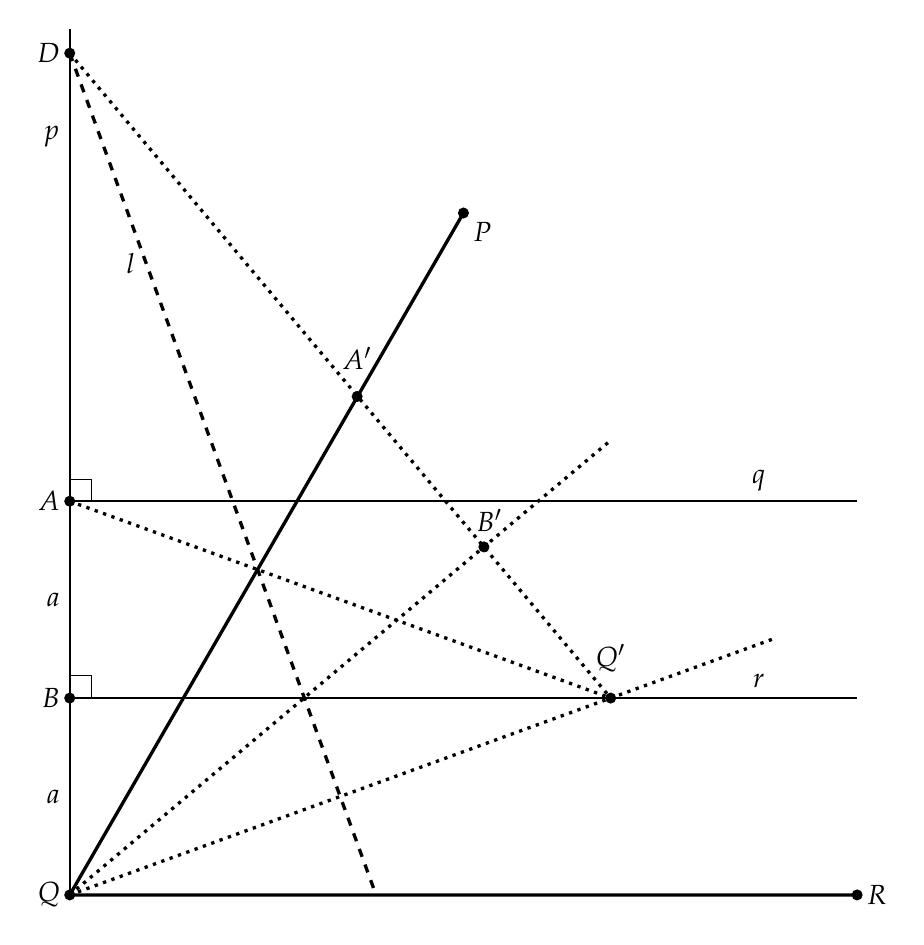
\begin{tikzpicture}[scale=1]

% Place points P, Q, R
\coordinate (P) at (60:10cm); %(5,8.67);
\coordinate (Q) at (0,0);
\coordinate (R) at (10,0);
\fill (P) circle (2pt) node[below right] {$P$};
\fill (Q) circle (2pt) node[left] {$Q$};
\fill (R) circle (2pt) node[right] {$R$};

% Draw PQR
\draw [very thick] (P)  -- (Q) -- (R);

% Draw perpendicular to QR
\draw [thick] (Q) -- node[left,very near end] {$p$} +(0,11);

% Draw parallel to QR and parallel halfway
\coordinate (A) at (0,5);
\coordinate (B) at (0,2.5);
\draw [thick] (A) -- node[above,very near end] {$q$} +(10,0);
\draw [thick] (B) -- node[above,very near end] {$r$} +(10,0);
\fill (A) circle (2pt) node[left] {$A$};
\fill (B) circle (2pt) node[left] {$B$};
\path (Q) -- node[left] {$a$} (B) -- node[left] {$a$} (A);
\draw (A) rectangle +(8pt,8pt);
\draw (B) rectangle +(8pt,8pt);

% Tangent line y = -2.75x + 10.69

% Draw fold
\coordinate (D) at (0,10.69);
\coordinate (fold-x) at (3.89,0);
\coordinate (AP) at (3.65,6.33);
\coordinate (QP) at (6.87,2.5);
\coordinate (BP) at (5.26,4.42);
\fill (D) circle (2pt) node[left] {$D$};
\fill (AP) circle (2pt) node[above,yshift=6pt] {$A'$};
\fill (QP) circle (2pt) node[above,yshift=6pt] {$Q'$};
\fill (BP) circle (2pt) node[above,xshift=2pt,yshift=2pt] {$B'$};
\draw [very thick,dashed] (D) -- node[left,near start] {$l$} (fold-x);

% Draw line of reflections
\draw [very thick, dotted] (D) -- (QP);

% Draw trisecting lines
\draw [very thick,dotted] (Q) -- ($(Q)!1.3!(QP)$);
\draw [very thick,dotted] (Q) -- ($(Q)!1.3!(BP)$);

% Complete triangle
\draw [very thick,dotted] (A) -- (QP);

\end{tikzpicture}
\end{center}
נתונה זווית חדה
$\angle PQR$,
יהי הקו
$p$
ניצב ל-%
$\overline{QR}$
ב-%
$Q$.
יהי הקו
$q$
ניצב ל-%
$p$
ב-% 
$A$
שחותך את
$\overline{PQ}$,
ויהי הקו
$r$
ניצב ל-%
$p$
ב-%
$B$
במחצית הדרך בן
$Q$
ו-%
$A$.

לפי אקסיומה 
$6$
בנה קיפול
$l$
המניח את 
$A$
על
$\overline{PQ}$ 
בנקודה
$A'$,
ומניח את
$Q$
על
$r$
בנקודה
$Q'$.
נסמן ב--%
$B'$
את השיקוף של 
$B$
מסביב ל-%
$l$.

בנה את הקווים
$\overline{QB'}$
ו-%
$\overline{QQ'}$.
טיעון: הזוויות
$\angle PQB'$, $\angle B'QQ'$, $\angle Q'QR$
מחלקות לשלושה חלקים את הזווית
$\angle PQR$.

\subsection{הוכחה ראשונה}

\begin{center}
\selectlanguage{english}
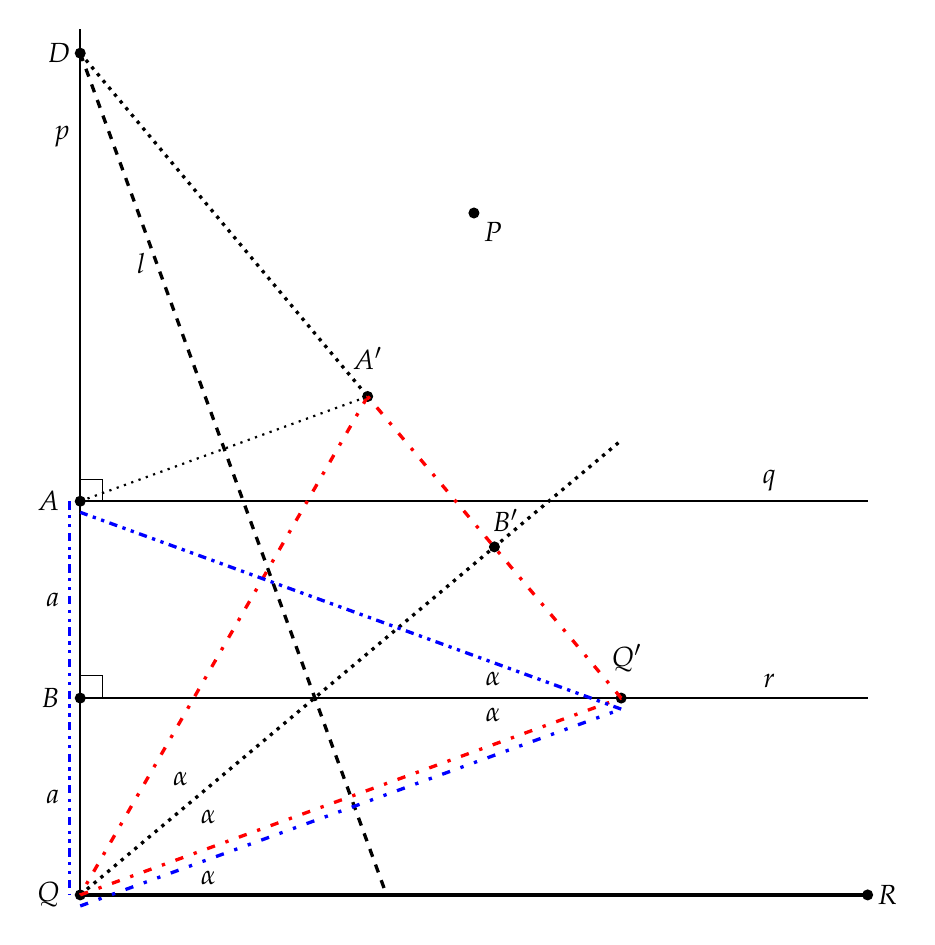
\begin{tikzpicture}[scale=1]

% Place points P, Q, R
\coordinate (P) at (60:10cm);
\coordinate (Q) at (0,0);
\coordinate (R) at (10,0);
\fill (P) circle (2pt) node[below right] {$P$};
\fill (Q) circle (2pt) node[left,xshift=-4pt] {$Q$};
\fill (R) circle (2pt) node[right] {$R$};

% Draw PQR
\draw [very thick] (Q) -- (R);

% Draw perpendicular to QR
\draw [thick] (Q) -- node[left,very near end] {$p$} +(0,11);

% Draw parallel to QR and parallel halfway
\coordinate (A) at (0,5);
\coordinate (B) at (0,2.5);
\draw [thick] (A) -- node[above,very near end] {$q$} +(10,0);
\draw [thick] (B) -- node[above,very near end] {$r$} +(10,0);
\fill (A) circle (2pt) node[left,xshift=-4pt] {$A$};
\fill (B) circle (2pt) node[left,xshift=-4pt] {$B$};
\path (Q) -- node[left,xshift=-4pt] {$a$} (B) -- node[left,xshift=-4pt] {$a$} (A);
\draw (A) rectangle +(8pt,8pt);
\draw (B) rectangle +(8pt,8pt);

% Tangent line y = -2.75x + 10.69

% Draw fold
\coordinate (D) at (0,10.69);
\coordinate (fold-x) at (3.89,0);
\coordinate (AP) at (3.65,6.33);
\coordinate (QP) at (6.87,2.5);
\coordinate (BP) at (5.26,4.42);
\fill (D) circle (2pt) node[left] {$D$};
\fill (AP) circle (2pt) node[above,yshift=6pt] {$A'$};
\fill (QP) circle (2pt) node[above,xshift=2pt,yshift=6pt] {$Q'$};
\fill (BP) circle (2pt) node[above,xshift=4pt,yshift=2pt] {$B'$};
\draw [very thick,dashed] (D) -- node[left,near start] {$l$} (fold-x);
	
% Draw line of reflections
\draw [very thick, dotted] (D) -- (AP);

% Draw trisecting lines
\draw [very thick,dotted] (Q) -- ($(Q)!1.3!(BP)$);

\draw [very thick,loosely dash dot,red] (Q) -- (QP);
\draw [very thick,loosely dash dot,red] (QP) -- (AP);
\draw [very thick,loosely dash dot,red] (AP) -- (Q);
\draw [very thick,loosely dash dot dot,blue] ($(Q)+(0,-4pt)$) -- ($(QP)+(0,-4pt)$);
\draw [very thick,dash dot dot,blue] ($(QP)+(0,-4pt)$) -- ($(A)+(0,-4pt)$);
\draw [very thick,dash dot dot,blue] ($(A)+(-4pt,0)$) -- ($(Q)+(-4pt,0)$);

\draw [thick,dotted] (A) -- (AP);

\node[left,xshift=-40pt,yshift=7pt] at (QP) {$\alpha$};
\node[left,xshift=-40pt,yshift=-6pt] at (QP) {$\alpha$};
\node[right,xshift=40pt,yshift=6pt] at (Q) {$\alpha$};
\node[right,xshift=40pt,yshift=28pt] at (Q) {$\alpha$};
\node[right,xshift=30pt,yshift=42pt] at (Q) {$\alpha$};

\end{tikzpicture}
\end{center}

הנקודות
$A', B', Q'$
הן שיקופים סביב אותו קו 
$l$
של הנקודות
$A,B,Q$
הנמצאות על קו אחד
$\overline{DQ}$,
ולכן גם הן נמצאות על קטע קו אחד
$\overline{DQ'}$.
לפי הבנייה,
$\overline{AB}=\overline{BQ}$, $\overline{BQ'}$
ניצב ל-%
$AQ$
ו-%
$\overline{BQ'}$
הוא צלע משותף, ולכן
$\triangle ABQ'\cong \triangle QBQ'$ 
לפי צלע-זווית-צלע. מכאן ש:
$\angle AQ'B=\angle QQ'B=\alpha$,
כי
$\overline{Q'B}$
הוא האנך האמצעי של המשולש שווי-שוקיים
$\triangle AQ'Q$.

לפי זוויות מתחלפות,
$\angle Q'QR=\angle QQ'B=\alpha$.

לפי שיקוף,
$\triangle AQ'Q\cong \triangle A'QQ'$.\footnote{%
שני המשולשים מודגשים על ידי קווים שונים של מקפים ונקודות, וכן על ידי הצבעים אדום וכחול.%
}
\begin{quote}
הוכחה: הקיפול
$l$
הוא האנך האמצעי של 
$\overline{AA'}$
וגם של
$\overline{QQ'}$;
בנה ניצבים מ-%
$A$
ו-%
$A'$
ל-%
$\overline{QQ'}$;
אזי
$\overline{AQ}=\overline{A'Q'}$
לפי משולשים ישר זווית חופפים.
$\overline{AA'Q'Q}$
הוא טרפז שווי-שוקיים כך שהאלכסונים שווים
$\overline{AQ'}=\overline{A'Q}$.
\end{quote}
מכאן ש-%
$\overline{QB'}$,
השיקוף של
$\overline{Q'B}$,
הוא האנך האמצעי של משולש שווי-שוקיים
$\triangle A'QQ'$,
ו-%
$\angle A'QB'=\angle Q'QB'=\angle QQ'B=\alpha$.

\subsection{הוכחה שנייה}

\begin{center}
\selectlanguage{english}
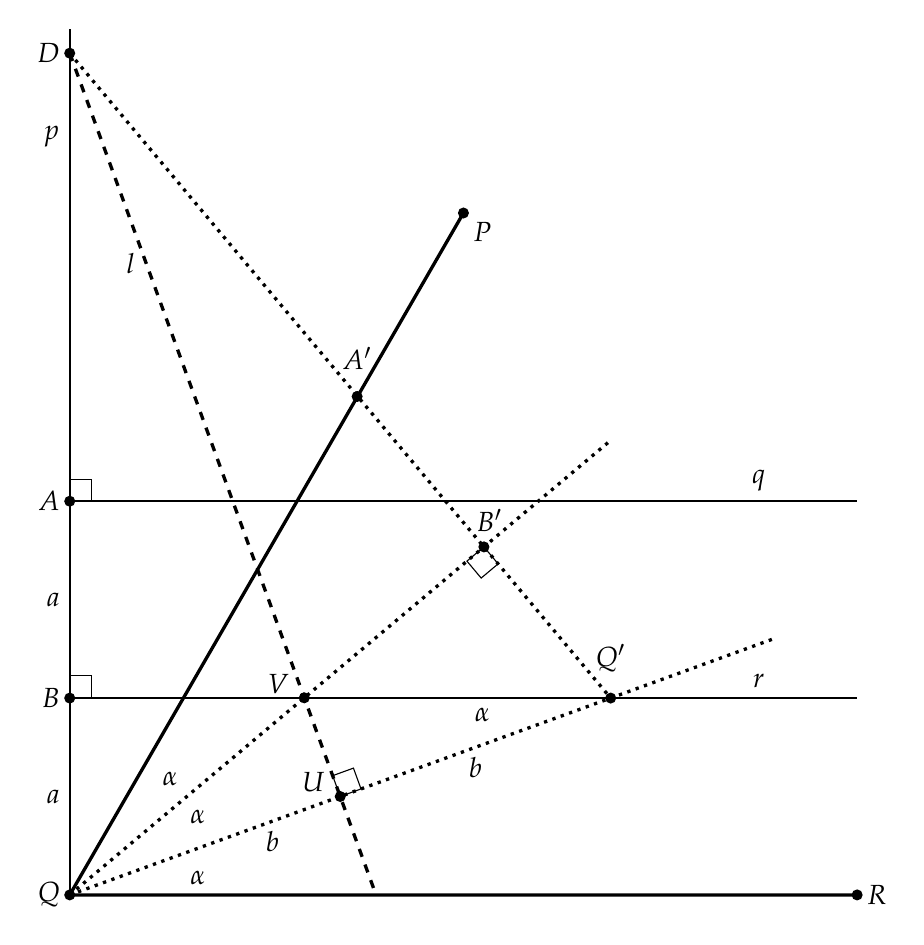
\begin{tikzpicture}[scale=1]

% Place points P, Q, R
\coordinate (P) at (60:10cm); %(5,8.67);
\coordinate (Q) at (0,0);
\coordinate (R) at (10,0);
\fill (P) circle (2pt) node[below right] {$P$};
\fill (Q) circle (2pt) node[left] {$Q$};
\fill (R) circle (2pt) node[right] {$R$};

% Draw PQR
\draw [very thick] (P)  -- (Q) -- (R);

% Draw perpendicular to QR
\draw [thick] (Q) -- node[left,very near end] {$p$} +(0,11);

% Draw parallel to QR and parallel halfway
\coordinate (A) at (0,5);
\coordinate (B) at (0,2.5);
\draw [thick] (A) -- node[above,very near end] {$q$} +(10,0);
\draw [thick] (B) -- node[above,very near end] {$r$} +(10,0);
\fill (A) circle (2pt) node[left] {$A$};
\fill (B) circle (2pt) node[left] {$B$};
\path (Q) -- node[left] {$a$} (B) -- node[left] {$a$} (A);
\draw (A) rectangle +(8pt,8pt);
\draw (B) rectangle +(8pt,8pt);

% Tangent line y = -2.75x + 10.69

% Draw fold
\coordinate (D) at (0,10.69);
\coordinate (fold-x) at (3.89,0);
\coordinate (AP) at (3.65,6.33);
\coordinate (QP) at (6.87,2.5);
\coordinate (BP) at (5.26,4.42);
\fill (D) circle (2pt) node[left] {$D$};
\fill (AP) circle (2pt) node[above,yshift=6pt] {$A'$};
\fill (QP) circle (2pt) node[above,yshift=6pt] {$Q'$};
\fill (BP) circle (2pt) node[above,xshift=2pt,yshift=2pt] {$B'$};
\draw [very thick,dashed,name path=fold] (D) -- node[left,near start] {$l$} (fold-x);

% Draw line of reflections
\draw [very thick, dotted] (D) -- (QP);

% Draw trisecting lines
\draw [very thick,dotted,name path=Qr] (Q) -- ($(Q)!1.3!(QP)$);
\draw [very thick,dotted,name path=Qq] (Q) -- ($(Q)!1.3!(BP)$);

% Draw indications of right angles
\draw[rotate=-140] (BP) rectangle +(8pt,8pt);
\path [name intersections = {of = fold and Qr, by = {U}}];
\fill (U) circle (2pt) node[above left,xshift=-2pt,yshift=-2pt] {$U$};
\draw[rotate=20] (U) rectangle +(8pt,8pt);
\path [name intersections = {of = fold and Qq, by = {V}}];
\fill (V) circle (2pt) node[above left,xshift=-2pt,yshift=-2pt] {$V$};

\path (Q) -- node[below,near end] {$b$} (U);
\path (U) -- node[below] {$b$} (QP);

\node[left,xshift=-40pt,yshift=-6pt] at (QP) {$\alpha$};
\node[right,xshift=40pt,yshift=6pt] at (Q) {$\alpha$};
\node[right,xshift=40pt,yshift=28pt] at (Q) {$\alpha$};
\node[right,xshift=30pt,yshift=42pt] at (Q) {$\alpha$};
\end{tikzpicture}
\end{center}

הקו
$l$
הוא קיפול, ולכן הוא האנך האמצעי של
$\overline{QQ'}$.
סמן ב-%
$U$
את נקודת החיתוך של
$l$
עם
$\overline{QQ'}$,
וסמן ב-%
$V$
את נקודת החיתוך שלו עם
$\overline{QB'}$.
$\triangle VUQ\cong \triangle VUQ'$
לפי צלע-זווית-צלע כי:
$\overline{VU}$
הוא צלע משותף, הזוויות ב-%
$U$
הן זוויות ישרות, ו-%
$\overline{QU}=\overline{Q'U}=b$.
מכאן ש-%
$\angle VQU=\angle VQ'U=\alpha$
ו-%
$\angle Q'QR=\angle VQ'U=\alpha$
לפי זוויות מתחלפות.

כמו בהוכחה הראשונה, הנקודות
$A', B', Q'$
הן כולן שיקופים סביב
$l$,
לכן הן כולן נמצאות על קטע קו אחד
$\overline{DQ'}$,
ו-%
$\overline{A'B'}=\overline{AB}=\overline{BQ}=\overline{B'Q'}=a$.
מכאן ש-%
$\triangle A'B'Q\cong\triangle Q'B'Q$
ו-%
$\angle A'QB'=\angle Q'QB'=\alpha$.


\newpage

\section{הבנייה של
\L{Martin}
לחלוקת זווית לשלושה חלקים%
}\label{s.tri2}

\subsection{הבנייה}

\begin{center}
\selectlanguage{english}
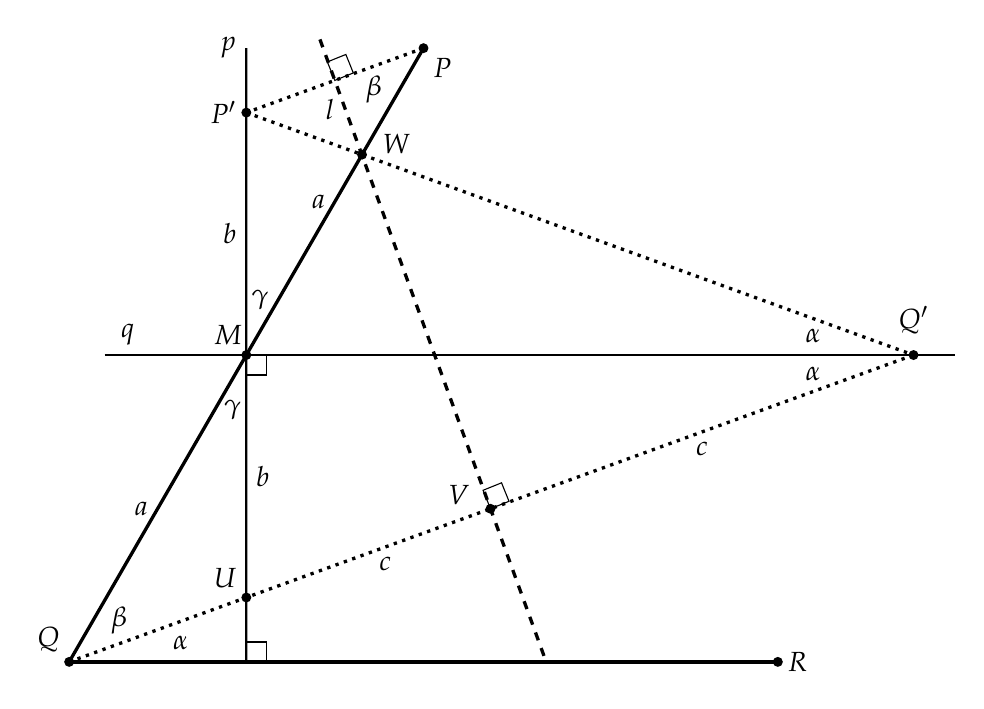
\begin{tikzpicture}[scale=.9]

% Place points P, Q, R
\coordinate (P) at (60:10cm); %(5,8.67);
\coordinate (Q) at (0,0);
\coordinate (R) at (10,0);
\fill (P) circle (2pt) node[below right] {$P$};
\fill (Q) circle (2pt) node[above left] {$Q$};
\fill (R) circle (2pt) node[right] {$R$};

% Draw PQR
\draw [very thick] (R)  -- (Q);
\draw [very thick,name path=pq] (Q) -- (P);

% M is the midpoint of PQ
\coordinate (M) at (2.5, 4.33);
\fill (M) circle (2pt) node[above left,xshift=2pt] {$M$};
\draw [rotate=-90] (M) rectangle +(8pt,8pt);

% Drop a perpendicular from M to QR and extend the line upwards
% This is the given line p
\coordinate (pQR) at (M |- Q);
\draw [thick,name path=p] (pQR) --
   node[left, very near end,yshift=28pt] {$p$}
   ($(pQR)!2!(M)$);
\draw (pQR) rectangle +(8pt,8pt);

% Construct q perpendicular to p through M
\draw [thick,name path=q] ($(M)+(-2,0)$) --
   node[above, very near start,xshift=-30pt] {$q$}
   ($(M)+(10,0)$);

% Construct the fold line t
% Its equation is y = -2.75x + 18.51, as obtained from Geogebra
\coordinate (t1) at (6.7,.085);
\coordinate (t2) at (3.5,8.89);
\draw [very thick,dashed,name path=t] (t1) --
   node[very near end,left] {$l$}
   (t2);

% Construct a perpendicular to t through P
\coordinate (perp-p) at ($(t1)!(P)!(t2)$);
\path [name path=perp-p] (P) -- ($(P)!2.5!(perp-p)$);

% Get its intersection with t denoted Pt
% and its intersection with p named PP
\path [name intersections = {of = t and perp-p, by = {Pt}}];
\path [name intersections = {of = p and perp-p, by = {PP}}];
\fill (PP) circle(2pt) node[left] {$P'$};
\draw [rotate=22] (Pt) rectangle +(8pt,8pt);

% Draw PT
\draw [very thick,dotted] (P) -- (PP);

% Construct a perpendicular to t through Q
\coordinate (perp-q) at ($(t1)!(Q)!(t2)$);
\path[name path=perp-q] (Q) -- ($(Q)!2.1!(perp-q)$);

% Get its intersection with t denoted V
% and its intersection with q denoted S=Q'
\path [name intersections = {of = t and perp-q, by = {V}}];
\path [name intersections = {of = q and perp-q, by = {QP}}];
\fill (QP) circle(2pt) node[above,yshift=4pt] {$Q'$};
\fill (V) circle(2pt) node[above left,xshift=-4pt,yshift=-2pt] {$V$};
\draw [rotate=22] (V) rectangle +(8pt,8pt);

% Draw Q QP
\draw [very thick,dotted,name path=qs] (Q) -- (QP);

% Get the intersection of QS with p denoted U
\path [name intersections = {of = p and qs, by = {U}}];
\fill (U) circle(2pt) node[above left] {$U$};

% Draw PP QP
\draw [very thick,dotted,name path=ts] (PP) -- (QP);

% Get its intersection with QP denoted W
\path [name intersections = {of = ts and pq, by = {W}}];
\fill (W) circle(2pt) node[right,xshift=4pt,yshift=4pt] {$W$};

% Label line segments
\path (P) -- node[left] {$a$} (M);
\path (M) -- node[left]  {$a$} (Q);
\path (PP) -- node[left]  {$b$} (M);
\path (M) -- node[right] {$b$} (U);
\path (Q) -- node[below,near end] {$c$} (V);
\path (V) -- node[below] {$c$} (QP);

% Label angles
\node [xshift=5pt,yshift=20pt]        at (M) {$\gamma$};
\node [xshift=-5pt,yshift=-20pt]      at (M) {$\gamma$};
\node [xshift=18pt,yshift=15pt]       at (Q) {$\beta$};
\node [xshift=-18pt,yshift=-15pt]     at (P) {$\beta$};
\node [left,xshift=-30pt,yshift=7pt]  at (QP) {$\alpha$};
\node [left,xshift=-30pt,yshift=-7pt] at (QP) {$\alpha$};
\node [right,xshift=34pt,yshift=7pt]  at (Q) {$\alpha$};
\end{tikzpicture}
\end{center}

נתונה זווית חדה
$\angle PQR$,
תהי
$M$
נקודת האמצע של
$\overline{PQ}$.
בנה
$p$
ניצב ל-%
$\overline{QR}$
העובר דרך
$M$
ובנה
$q$
ניצב ל-%
$p$
העובר דרך 
$M$.
$q$
מקביל ל-%
$\overline{QR}$.

לפי אקסיומה $6$, בנה קיפול
$l$
המניח את
$P$
ב-%
$P'$
על
$p$,
ומניח את
$Q$
ב-%
$Q'$
על
$q$.
ייתכן שקיים מספר קיפולים מתאימים; בחר את הקיפול החותך את
$\overline{PM}$.

בנה את קטעי הקו
$\overline{PP'}$
ו-%
$\overline{QQ'}$.
סמן ב-%
$U$
את נקודת החיתוך של
$\overline{QQ'}$
עם
$p$,
וסמן ב-%
$V$
את נקודת החיתוך שלו עם
$l$.
סמן ב-%
$W$
את החיתוכים של 
$\overline{PQ}$
ו-%
$\overline{P'Q'}$
עם
$l$.\footnote{%
לא ברור מאליו ש-%
$\overline{PQ}$
ו-%
$\overline{P'Q'}$
חותכים את
$l$
באותה נקודה. 
$\triangle PP'W\sim\triangle QQ'W$
כך שהגבהים מחלקים את הזוויות 
$\angle PWP', \angle QWQ'$
בצורה דומה וחייבים להיות על אותו קו.%
}

\subsection{הוכחה}

$\triangle QMU\cong \triangle PMP'$
לפי זווית-צלע-זווית:
$\angle P'PM=\angle UQM=\beta$
לפי זוויות מתחלפות;
$\overline{QM}=\overline{MP}=a$
כי 
$M$
היא נקודת האמצע של
$\overline{PQ}$;
$\angle QMU=\angle PMP'$
הן זוויות קודקודיות. מכאן ש-%
$\overline{P'M}=\overline{MU}=b$.

$\triangle P'MQ'\cong\triangle UMQ'$
לפי צלע-זוויות-צלע: הראנו ש-%
$\overline{P'M}=\overline{MU}=b$;
הזוויות ב-%
$M$
הן זוויות ישרות; 
$\overline{MQ'}$
הוא צלע משותף. הגובה של המשולש שווה-שוקיים 
$\triangle P'Q'U$ 
הוא חוצה הזווית
$\angle P'Q'U$
ולכן
$\angle P'Q'M=\angle UQ'M=\alpha$.


$\triangle QWV\cong\triangle Q'WV$
לפי צלע-זווית-צלע:
$\overline{QV}=\overline{VQ'}=c$
והזוויות ב-%
$V$
הן זוויות ישרות כי הקיפול הוא האנך אמצעי של
$\overline{QQ'}$; $\overline{VW}$
הוא צלע משותף. מכאן ש-%
$\angle WQV=\beta=\angle WQ'V=2\alpha$.
הראנו ש-%
$\angle PQR = \beta + \alpha = 2\alpha+\alpha=3\alpha$
ולכן
$\angle Q'QR$
היא שליש מ-%
$\angle PQR$.

% !TeX root = origami-math-he.tex

%%%%%%%%%%%%%%%%%%%%%%%%%%%%%%%%%%%%%%%%%%%%%%%%%%%%%%%%%%%%%%%%
\chapter{הכפלת קוביה}\label{c.cube}

\section{%
הבנייה של 
\L{Messer}
להכפלת קוביה}%
\label{s.cube1}

לקוביה בנפח 
$V$
צלעות באורך
$\sqrt[3]{V}$.
נפח קוביה שנפחה פי שניים הוא
 $2\cdot V$,
 כך שיש לבנות קטע קו באורך
$\sqrt[3]{2\cdot V}=\sqrt[3]{2}\cdot \sqrt[3]{V}$.
אם נוכל לבנות קטע קו באורך
$\sqrt[3]{2}$,
נוכל להכפיל באורך הנתון
$\sqrt[3]{V}$
כדי להכפיל את נפח הקוביה.

\subsection{חלוקת קטע קו לשלוש}

\L{Lang \cite{lang}}
מביא בניות יעילות עבור שברים רציונליים של אורכו של צלע של )דף נייר שהוא( ריבוע. כאן עלינו לחלק צלע של ריבוע לשלושה חלקים.

תחילה, קפל את הריבוע לחצי כדי למצוא את הנוקדה
$J=(1,1/2)$.
אחר כך, בנה את קטעי הקו
$\overline{AC}$
ו-%
$\overline{BJ}$.
\begin{center}
\selectlanguage{english}
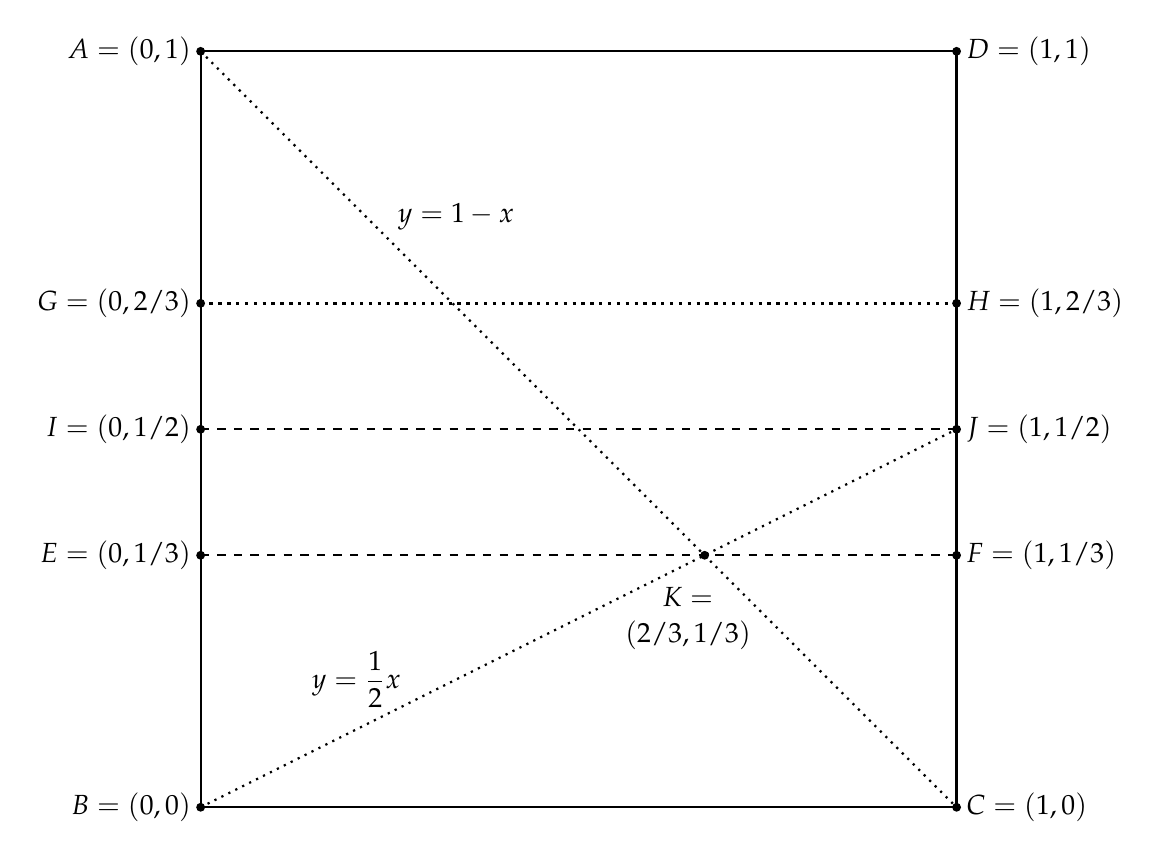
\begin{tikzpicture}[scale=.8]
% Draw square
\coordinate (A) at (0,12);
\coordinate (B) at (0,0);
\coordinate (C) at (12,0);
\coordinate (D) at (12,12);

\fill (A) circle (2pt) node[left]  {$A=(0,1)$};
\fill (B) circle (2pt) node[left]  {$B=(0,0)$};
\fill (C) circle (2pt) node[right] {$C=(1,0)$};
\fill (D) circle (2pt) node[right] {$D=(1,1)$};

\draw [thick] (A)  -- (B) -- (C) -- (D) -- cycle;

% Divide a side in half

\coordinate (M)  at (0,6);
\coordinate (N) at (12,6);
\fill (M) circle (2pt) node[left] {$I=(0,1/2)$};
\fill (N) circle (2pt) node[right] {$J=(1,1/2)$};
\draw [thick,dashed] (M) -- (N);


\draw [thick,dotted,name path=ac] (A) -- 
   node[near start,above,xshift=24pt] {$y=1-x$} (C);
\draw [thick,dotted,name path=be2] (B) -- 
   node[near start,above,xshift=-12pt,yshift=-2pt] {$y=\disfrac{1}{2}x$} (N);

\path [name intersections = {of = ac and be2, by = {I}}];
\fill (I) circle (2pt) 
   node[below,xshift=-6pt,yshift=-8pt] {$K=$}
   node[below,xshift=-6pt,yshift=-20pt] {$(2/3,1/3)$};

\coordinate (E)  at (0,4);
\coordinate (F) at (12,4);
\fill (E) circle (2pt) node[left] {$E=(0,1/3)$};
\fill (F) circle (2pt) node[right] {$F=(1,1/3)$};
\draw [thick,dashed] (E) -- (F);

\coordinate (G)  at (0,8);
\coordinate (H) at (12,8);
\fill (G) circle (2pt) node[left] {$G=(0,2/3)$};
\fill (H) circle (2pt) node[right] {$H=(1,2/3)$};
\draw [very thick,dotted] (G) -- (H);
\end{tikzpicture}
\end{center}
אפשר לחשב את הקואורדינטות של נקודה החיתוך 
$K$
על ידי פתרון של שתי המשוואות הללו:
\begin{form}{1.8}
y&=&1-x\\
y&=&\disfrac{1}{2}x\,.
\end{form}
הפתרון הוא:
$x=2/3, y=1/3$.

בנה את הקו
$\overline{EF}$
ניצב ל-%
$\overline{AB}$
כך שהוא עובר דרך 
$K$,
ובנה את 
$\overline{GH}$,
השיקוף של
$\overline{BC}$
סביב
$\overline{EF}$.
הצלע של הריבוע מחולק לשלושה חלקים.

\subsection{בניית $\sqrt[3]{2}$}

\begin{center}
\selectlanguage{english}
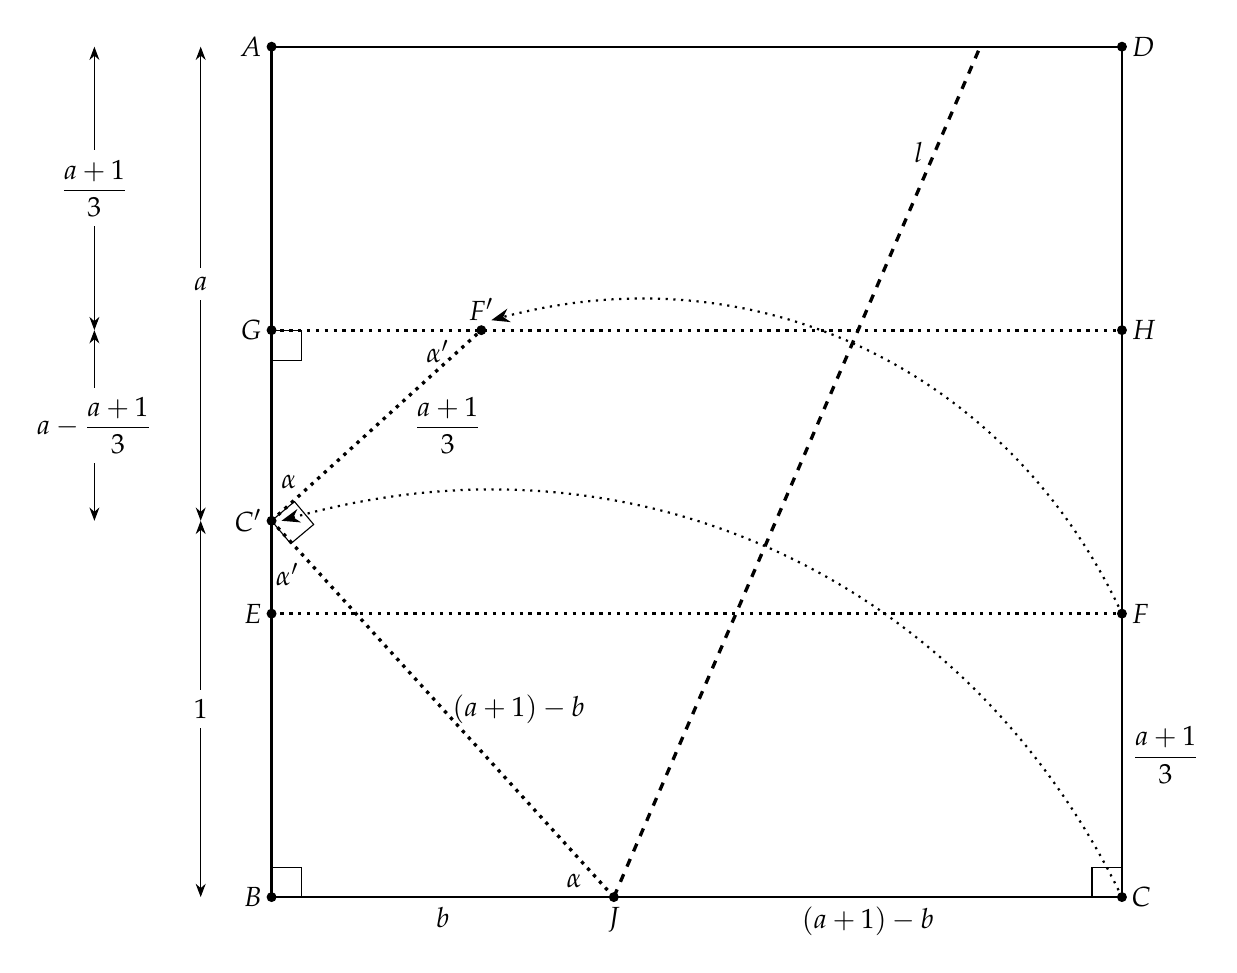
\begin{tikzpicture}[scale=.9]
% Draw and label square
\coordinate (A) at (0,12);
\coordinate (B) at (0,0);
\coordinate (C) at (12,0);
\coordinate (D) at (12,12);
\fill (A) circle (2pt) node[left]  {$A$};
\fill (B) circle (2pt) node[left]  {$B$};
\fill (C) circle (2pt) node[right] {$C$};
\fill (D) circle (2pt) node[right] {$D$};
\draw (B) rectangle +(12pt,12pt);
\draw[rotate=90] (C) rectangle +(12pt,12pt);
\draw [thick] (A)  -- (B) -- (C) -- (D) -- cycle;

% Draw line one-third from botton
\coordinate (E)  at (0,4);
\coordinate (F) at (12,4);
\fill (E) circle (2pt) node[left] {$E$};
\fill (F) circle (2pt) node[right] {$F$};
\draw [very thick,dotted,name path=ef] (E) -- (F);

% Draw line two-thirds from bottom
\coordinate (G)  at (0,8);
\coordinate (H) at (12,8);
\fill (G) circle (2pt) node[left] {$G$};
\fill (H) circle (2pt) node[right] {$H$};
\draw[rotate=-90] (G) rectangle +(12pt,12pt);
\draw [very thick,dotted] (G) -- (H);

% Draw reflections of C and F
\coordinate (CP) at (0,5.31);
\coordinate (FP) at (2.96,8);
\fill (CP) circle (2pt)
  node[left] {$C'$}
  node[above right,yshift=8pt] {$\alpha$}
  node[below right,xshift=-2pt,yshift=-12pt] {$\alpha'$};
\fill (FP) circle (2pt)
  node[above] {$F'$}
  node[below left,xshift=-8pt] {$\alpha'$};
\draw[rotate=-50] (CP) rectangle +(12pt,12pt);
\draw[very thick,dotted] (CP) -- (FP);

% Draw fold and fold arrows
% Tangent is y = 2.26x - 10.9
% Crosses x axis at (4.83,0)
\coordinate (J) at (4.83,0);
\fill (J) circle (2pt)
    node[below] {$J$}
    node[above left,xshift=-8pt] {$\alpha$};
\draw [very thick,dashed,name path=jd] (J) -- node[very near end,left] {$l$} (10,12);
\draw[thick,dotted,bend right=40,->] (C) to ($(CP)+(4pt,0)$);
\draw[thick,dotted,bend right=40,->] (F) to ($(FP)+(4pt,4pt)$);

% Draw hypotenuses of right triangles
\draw[very thick,dotted] (CP) -- (J);
\path (J)  -- (C);

% Labels on BC and hypotenuses
\path (CP) -- node[right] {$(a+1)-b$} (J);
\path (J)  -- node[below] {$(a+1)-b$} (C);
\path (B)  -- node[below] {$b$} (J);
\path (C)  -- node[right] {$\disfrac{a+1}{3}$} (F);
\path (CP) -- node[right,xshift=10pt] {$\disfrac{a+1}{3}$} (FP);

% Labels on AB
\draw[<->] ($(A)+(-1,0)$)    --
  node[fill=white] {$a$} ($(CP)+(-1,0)$);
\draw[<->] ($(CP)+(-1,0)$)   --
  node[fill=white] {$1$} ($(B)+(-1,0)$);
\draw[<->] ($(CP)+(-2.5,0)$) --
  node[fill=white] {$a-\disfrac{a+1}{3}$} ($(G)+(-2.5,0)$);
\draw[<->] ($(A)+(-2.5,0)$) --
  node[fill=white] {$\disfrac{a+1}{3}$} ($(G)+(-2.5,0)$);
\end{tikzpicture}
\end{center}

נמסן צלע של הריבוע 
$a+1$.
הבנייה תראה ש-%
$a=\sqrt[3]{2}$.

נשמתש באקסיומה $6$ כדי להניח את 
$C$
ב-%
$C'$
על
$\overline{AB}$,
ולהניח את
$F$
ב-%
$F'$
על
$\overline{GH}$.
סמן את נקודת החיתוך של הקיפול עם
$\overline{BC}$ 
ב-%
$J$,
וסמן את אורכו של
$\overline{BJ}$
ב-%
$b$.
האורך של קטע הקו 
$\overline{JC}$
הוא
$(a+1)-b$.

לאחר ביצוע הקיפול, קטע הקו
$\overline{JC}$
הוא שיקוף של קטע הקו
$\overline{JC'}$
מאותו אורך, וקטע הקו

$\overline{CF}$
הוא שיקוף של קטע הקו
$\overline{C'F'}$
באותו אורך. חישוב פשוט מראה שאורכו של
$\overline{GC'}$
הוא:
\begin{equation}
\selectlanguage{english}
a-\disfrac{a+1}{3}=\disfrac{2a-1}{3}\,.\label{eq.one-third}
\end{equation}
לבסוף,
$\angle FCJ$
היא זווית ישרה, לכן גם
$\angle F'C'J$ 
היא זווית ישרה.

$\triangle C'BJ$
הוא משולש ישר-זווית ולפי משפט פתגורוס:
\begin{form}{1.3}
1^2 + b^2 &=& ((a+1)-b)^2\\
%&=& a^2+2a+1 - 2(a+1)b + b^2\\
a^2+2a - 2(a+1)b&=&0\\
b&=&\disfrac{a^2+2a}{2(a+1)}\,.
\end{form}

$\angle GC'F' + \angle F'C'J + \angle JC'B = 180^\circ$
כי הם מרכיבים קו ישר
$\overline{GB}$.
נסמן
$\alpha=\angle GC'F'$.
אז:
\[
\angle JC'B=180^\circ - \angle F'C'J - \angle GC'F'= 180^\circ - 90^\circ - \angle GC'F' = 90^\circ-\angle GC'F = 90^\circ -\alpha\,.
\]
נסמן
$\alpha'=90^\circ-\alpha$.
המשולשים
$\triangle C'BJ$, $\triangle F'GC'$
הם משולשים ישר-זווית, ולכן 
$\angle C'JB=\alpha$
ו-%
$\angle C'F'G=\alpha'$.
מכאן שהמשולשים דומים וממשוואה%
~\L{\ref{eq.one-third}}
מתקבלת המשוואה:
\[
\disfrac{b}{(a+1)-b}=\disfrac{\disfrac{2a-1}{3}}{\disfrac{a+1}{3}}\,.
\]
נציב עבור
$b$:
\begin{form}{2}
\disfrac{\disfrac{a^2+2a}{2(a+1)}}{(a+1)-\disfrac{a^2+2a}{2(a+1)}}&=&\disfrac{2a-1}{a+1}\\
%\disfrac{a^2+2a}{(a+1)\cdot 2(a+1)-(a^2+2a)}&=&\disfrac{2a-1}{a+1}\\
\disfrac{a^2+2a}{a^2+2a +2}&=&\disfrac{2a-1}{a+1}\,.
%a^3+3a^2+2a&=&(2a-1)(a^2+2a+2)\,.
%&=&2a^3+3a^2+2a-2\,.
\end{form}
נפשט ונקבל
$a^3=2$
ו-%
$a=\sqrt[3]{2}$.



\newpage

\section{הבנייה של
\L{Beloch}
להכפלת קוביה%
}\label{s.cube2}

ב-%
$1936$
\L{Margharita P. Beloch}
נתנה הגדרה פורמלית לאקסיומה~$6$ )הנקרא לעתים הקיפול של
\L{Beloch}(.
היא הראתה שניתן להשמתמש באקסיומה כדי לפתור משוואות ממעלה שלוש. כאן אנחנו נביא את השיטה שלה להכפלת קוביה. נדון בפתרון של משוואות ממעלה שלוש בפרקים%
~\L{\ref{c.lill}, \ref{c.beloch}}.

\subsection{הבנייה}

נסמן את הנקודה
$(-1,0)$
ב-%
$A$
ואת הנקודה
$(0,-2)$
ב-%
$B$.
נסמן ב-%
$p$ 
את הקו 
$x=1$
וב-%
$q$
את הקו
$y=2$.
לפי אקסיומה $6$ ניתן לבנות קיפול 
$l$
המניח את
$A$
ב-%
$A'$
על 
$p$,
והמניח את
$B$
ב-%
$B'$
על
$q$.
נסמן ב-%
$Y$
את נקודת החיתוך של הקיפול עם ציר ה-%
$y$,
ונסמן ב-%
$X$
את נקודת החיתוך של הקיפול עם ציר ה-%
$x$.

\begin{center}
\selectlanguage{english}
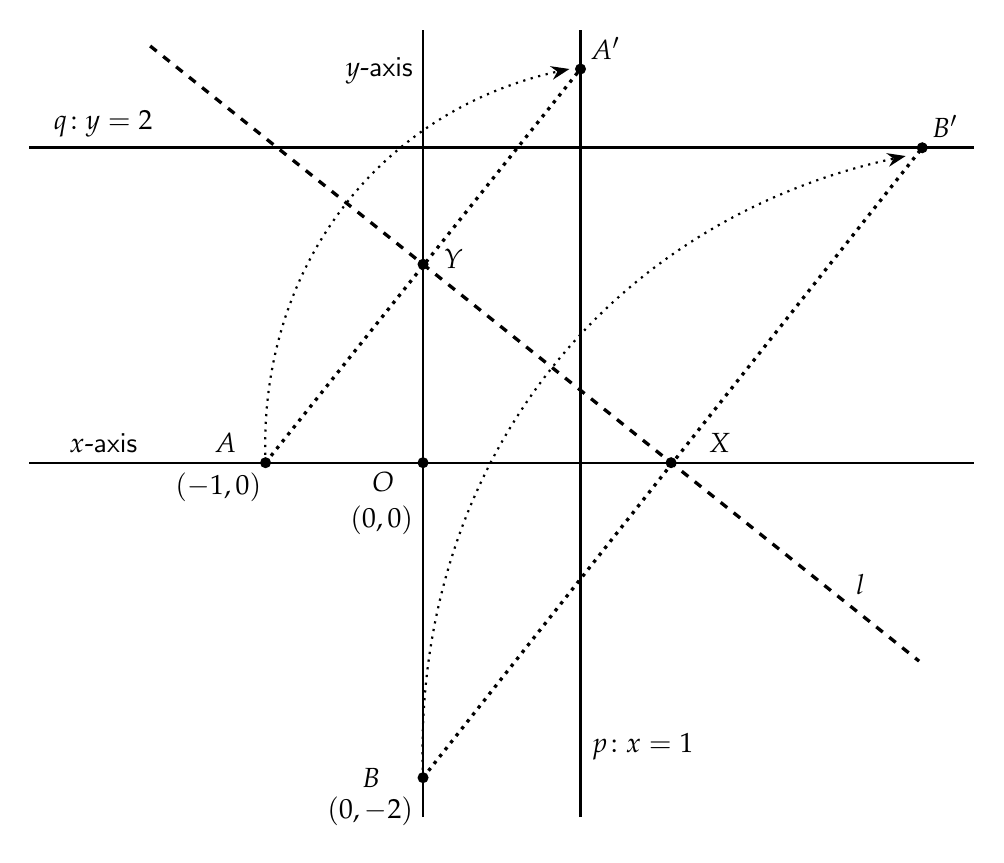
\begin{tikzpicture}[scale=1]
% Draw and label square
\coordinate (O) at (0,0);
\coordinate (A) at (-2,0);
\coordinate (B) at (0,-4);
\fill (O) circle (2pt)
  node[below left,xshift=-7pt] {$O$}
  node[below left,yshift=-12pt] {$(0,0)$};
\fill (A) circle (2pt)
  node[above left,xshift=-7pt] {$A$}
  node[below left,xshift=2pt,yshift=0pt] {$(-1,0)$};
\fill (B) circle (2pt)
  node[left,xshift=-12pt] {$B$}
  node[left,yshift=-12pt] {$(0,-2)$};

\draw[thick] (0,-4.5) --  node[very near end,above left,yshift=12pt] {$y$-\textsf{axis}} +(0,10);
\draw[thick] (-5,0)   -- node[very near start,above left] {$x$-\textsf{axis}} +(12,0);
\draw[very thick] (2,-4.5) -- node[very near start, right,yshift=-10pt] {$p\!:x=1$} +(0,10);
\draw[very thick] (-5,4) -- node[very near start, above,xshift=-16pt] {$q\!: y=2$} +(12,0);

\coordinate (AP) at (2,5);
\fill (AP) circle (2pt) node[above right] {$A'$};
\coordinate (BP) at (6.34,4);
\fill (BP) circle (2pt) node[above right] {$B'$};

% Tangent y = -0.8x + 1.26

% Exchanged X and Y 
\coordinate (X) at (0,2.52);
\coordinate (Y) at (3.15,0);
\fill (X) circle (2pt) node[right,xshift=4pt,yshift=2pt] {$Y$};
\fill (Y) circle (2pt) node[above right,xshift=10pt] {$X$};
\draw [very thick,dashed] ($(X)!-1.1!(Y)$) -- node[very near end,right,xshift=8pt] {$l$} ($(X)!2!(Y)$);

\draw [very thick,dotted] (A) -- (AP);
\draw [very thick,dotted] (B) -- (BP);

\draw[thick,dotted,bend left=40,->] (A) to ($(AP)+(-4pt,0)$);
\draw[thick,dotted,bend left=40,->] (B) to ($(BP)+(-6pt,-3pt)$);

\end{tikzpicture}
\end{center}

\newpage

\subsection{הוכחה}

נחלץ איור פשוט יותר:
\begin{center}
\selectlanguage{english}
\begin{tikzpicture}[scale=1]
\coordinate (O) at (0,0);
\coordinate (A) at (-2,0);
\coordinate (B) at (0,-4);
\fill (O) circle (2pt)
  node[below left,xshift=-7pt] {$O$};
\fill (A) circle (2pt)
  node[above left,xshift=-7pt] {$A$}
  node[above right,xshift=10pt] {$\alpha$};
\fill (B) circle (2pt)
  node[left,xshift=-12pt] {$B$}
  node[above right,yshift=12pt] {$\alpha'$};

\draw[thick] (0,-4.5) -- +(0,10);
\draw[thick] (-3,0)   -- +(8,0);

\coordinate (AP) at (2,5);
\fill (AP) circle (2pt) node[above right] {$A'$};
\coordinate (BP) at (6.34,4);
\fill (BP) circle (2pt) node[above right] {$B'$};

% Tangent y = -0.8x + 1.26

% Exchanged X and Y 
\coordinate (X) at (0,2.52);
\coordinate (Y) at (3.15,0);
\fill (X) circle (2pt)
  node[right,xshift=4pt,yshift=2pt] {$Y$}
  node[below right,yshift=-14pt] {$\alpha$}
  node[below left,xshift=2pt,yshift=-12pt] {$\alpha'$};
\fill (Y) circle (2pt)
  node[above right,xshift=10pt] {$X$}
  node[below left,xshift=-10pt] {$\alpha$}
  node[above left,xshift=-15pt] {$\alpha'$};
\draw [very thick,dashed] ($(X)!-.4!(Y)$) -- ($(X)!1.2!(Y)$);

\draw [very thick,dotted] (A) -- (AP);
\draw [very thick,dotted] (B) -- (BP);

\draw (0,0) rectangle +(10pt,10pt);
\draw[rotate=-130] (X) rectangle +(10pt,10pt);
\draw[rotate=-130] (Y) rectangle +(10pt,10pt);

\end{tikzpicture}
\end{center}
הקיפול הוא האנך האמצעי של
$\overline{AA'}$
ן-%
$\overline{BB'}$.
לכן
$\angle AYX$
ו-%
$\angle YXB$
הן זוויות ישר-זווית ו-%
$\overline{AA'}$ 
מקביל ל-%
$\overline{BB'}$.
לפי זוויות מתחלפות
$\angle XAO =\angle BYO=\alpha$.
אם זווית חדה אחת של משולש ישר-זווית היא
$\alpha$,
הזווית החדה השנייה היא
$90^\circ - \alpha$
שנסמן
$\alpha'$.
מכאן מתקבלים סימוני הזוויות האחרות באיור.

יש לנו שלושה משולשים דומים:
$\triangle AOY\sim \triangle YOX \sim \triangle XOB$.
קטעי קו
$\overline{OA}=1$, $\overline{OB}=2$
נתונים ולכן:
\begin{form}{2}
\disfrac{\overline{OY}}{\overline{OA}}=\disfrac{\overline{OX}}{\overline{OY}}=\disfrac{\overline{OB}}{\overline{OX}}\\
\disfrac{\overline{OY}}{1}=\disfrac{\overline{OX}}{\overline{OY}}=\disfrac{2}{\overline{OX}}\\
\overline{OY}^2=\overline{OX}=\disfrac{2}{\overline{OY}}\;,
\end{form}

מכאן ש-%
$\overline{OY}^3=2$
ו-%
$\overline{OY}=\sqrt[3]{2}$.

% !TeX root = origami-activities-en.tex

%%%%%%%%%%%%%%%%%%%%%%%%%%%%%%%%%%%%%%%%%%%%%%%%%%%%%%%%%%%%%%%%%%
%%%%%%%%%%%%%%%%%%%%%%%%%%%%%%%%%%%%%%%%%%%%%%%%%%%%%%%%%%%%%%%%%%
%%%%%%%%%%%%%%%%%%%%%%%%%%%%%%%%%%%%%%%%%%%%%%%%%%%%%%%%%%%%%%%%%%

\section*{Further reading}

Applications of origami \cite{lang-ted}. Mathematical theory of origami \cite{alperin,moti-origami}. History of origami \cite{history}. Paper folding \cite{lang,newton}.


\bibliographystyle{plain}
\bibliography{origami-activities-en}

% !TeX root = origami-math.tex

\appendix

\newpage

\section{GeoGebra links}\label{a.geo}

\begin{center}
\begin{tabular}{|l|l|}
\hline
Axiom 1& \url{https://www.geogebra.org/m/fq9d5hms}\\\hline
Axiom 2& \url{https://www.geogebra.org/m/fgmfss27}\\\hline
Axiom 3& \url{https://www.geogebra.org/m/ek3mqupw}\\\hline
Axiom 4& \url{https://www.geogebra.org/m/renzzbdg}\\\hline
Axiom 5& \url{https://www.geogebra.org/m/aszn9ywu}\\\hline
Axiom 6& \url{https://www.geogebra.org/m/bxe5e5ku}\\\hline
Axiom 7& \url{https://www.geogebra.org/m/yeq5gmeg}\\\hline
Abe's trisection & \url{https://www.geogebra.org/m/dxrcvjam}\\\hline
Martin's trisection & \url{https://www.geogebra.org/m/caky7edd}\\\hline
Messer's doubling of the cube & \url{https://www.geogebra.org/m/mrcwjqh8}\\\hline
Beloch's doubling of the cube & \url{https://www.geogebra.org/m/enzmmwua}\\\hline
\end{tabular}
\end{center}
Due to a bug in Geogebra, in projects that use Axiom~6, points defined by reflection around the common tangent are not saved or are saved incorrectly.

\section{Derivation of the trigonometric identities}\label{a.tangent}

The trigonometric identifies for tangent used in the proof of Axiom 3 can be derived from identifies for the sine and cosine:

\begin{form}{2.2}
\tan (\theta_1+\theta_2) &=& \disfrac{\sin(\theta_1+\theta_2)}{\cos(\theta_1+\theta_2)}\\
&=&\disfrac{\sin\theta_1\cos\theta_2+\cos\theta_1\sin\theta_2}{\cos\theta_1\cos\theta_2-\sin\theta_1\sin\theta_2}\\
&=&\disfrac{\sin\theta_1+\cos\theta_1\tan\theta_2}{\cos\theta_1-\sin\theta_1\tan\theta_2}\\
&=&\disfrac{\tan\theta_1+\tan\theta_2}{1-\tan\theta_1\tan\theta_2}\,.
\end{form}

We use this formula with $\theta=(\theta/2)+(\theta/2)$ to obtain a quadratic equation in $\tan(\theta/2)$:
\begin{form}{2.2}
\tan \theta=\disfrac{\tan(\theta/2)+\tan(\theta/2)}{1-\tan^2(\theta/2)}\\
\tan\theta \,(\tan(\theta/2))^2 \;+\; 2\,(\tan (\theta/2)) \;-\;\tan \theta = 0\,.
\end{form}
Its solutions are:
\[
\tan(\theta/2) = \disfrac{-1\pm\sqrt{1+\tan^2\theta}}{\tan\theta}\,.
\]

\newpage

\section{Parabolas}\label{a.parabola}


Students are usually introduced to parabolas as the graphs of second degree equations:
\[
y=ax^2+bx+c\,.
\]
However, parabolas can be defined geometrically: given a point, the \emph{focus}, and a line, the \emph{directrix}, the locus of points equidistant from the focus and the directrix defines a parabola.


The following diagram shows the focus---the large point at $p=(0,f)$, and the directrix---the thick line whose equation is $y=-f$. The resulting parabola is shown as a dotted curve. Its vertex $p_2$ is at the origin of the axes.

%\begin{figure}[H]
\begin{center}
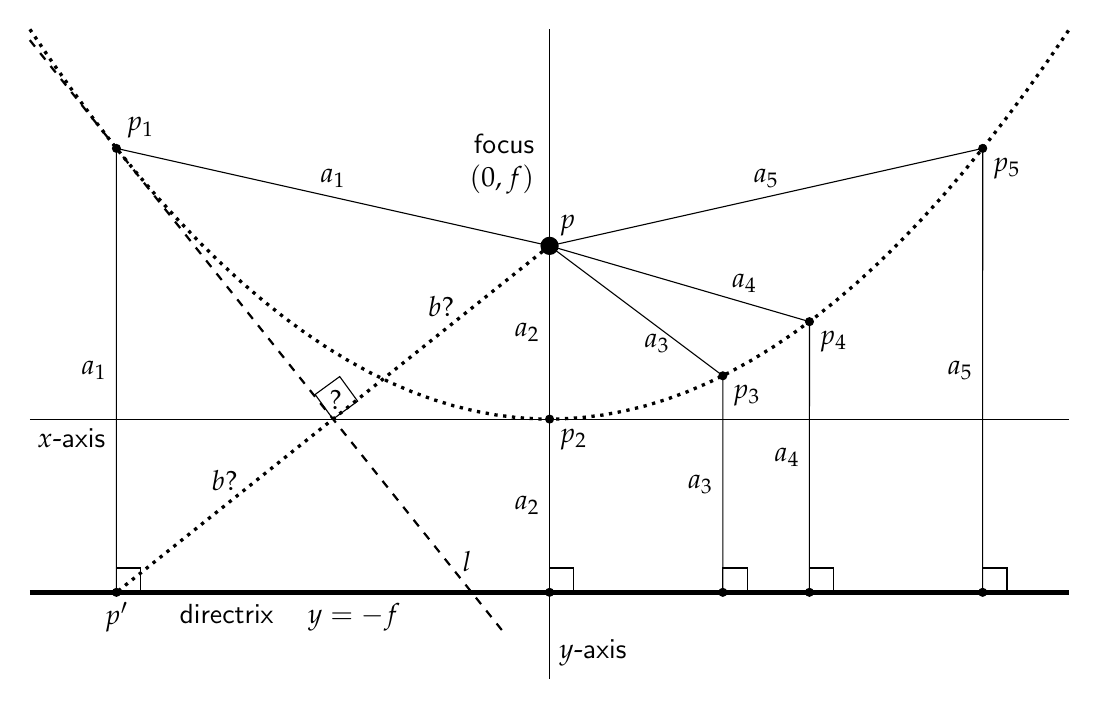
\begin{tikzpicture}[scale=1.1]
\draw (-6,0) -- node[very near start,below,xshift=-32pt] {$x$-\textsf{axis}} (6,0);
\draw (0,-3) -- node[very near start,right,yshift=-20pt] {$y$-\textsf{axis}} (0,4.5);
\draw[ultra thick] (-6,-2) -- node[near start,below] {\textsf{directrix} $\quad y=-f$} (6,-2);
\draw[domain=-6:6,samples=50,very thick,dotted] plot (\x,{\x*\x/8});
\coordinate (F) at (0,2);
\fill (F) circle (3pt) node[above left,xshift=-2pt,yshift=15pt] {$(0,f)$} node[above left,xshift=-2pt,yshift=30pt] {\textsf{focus}} node[above right] {$p$};
\fill (0,0) circle (1.5pt) node[below right] {$p_2$};
\fill (0,-2) circle (1.5pt);
\fill (2,-2) circle (1.5pt);
\fill (3,-2) circle (1.5pt);
\fill (5,-2) circle (1.5pt);
\coordinate (FP) at (-5,-2);
\fill (FP) circle (1.5pt) node[below] {$p'$};
\coordinate (F1) at (2,.5);
\fill (F1) circle (1.5pt) node[below right] {$p_3$};
\coordinate (F2) at (3,1.125);
\fill (F2) circle (1.5pt) node[below right] {$p_4$};
\coordinate (F3) at (5,3.125);
\fill (F3) circle (1.5pt) node[below right] {$p_5$};
\coordinate (F4) at (-5,3.125);
\fill (F4) circle (1.5pt) node[above right] {$p_1$};
\draw (F) -- node[left] {$a_2$} (0,0) -- node[left] {$a_2$} (0,-2);
\draw (F) -- node[near end,left] {$a_3$} (F1) -- node[left] {$a_3$} (2,-2);
\draw (F) -- node[near end,above] {$a_4$} (F2) -- node[left] {$a_4$} (3,-2);
\draw (F) -- node[above] {$a_5$} (F3) -- node[left] {$a_5$} (5,-2);
\draw (F) -- node[above] {$a_1$} (F4) -- node[left] {$a_1$} (FP);
\draw[thick,dashed] ($(F4)!-.4!(-2.5,0)$) -- node[very near end,right,xshift=2pt] {$l$} ($(F4)!1.8!(-2.5,0)$);
\draw[very thick,dotted] (F) -- (FP);
\coordinate (H) at (-2.5,0);
\node[above,xshift=1pt] at (H) {$?$};
\draw[rotate=36] (H) rectangle +(10pt,10pt);
\path (FP) -- node[above,yshift=2pt] {$b?$} (H) -- node[above,yshift=2pt] {$b?$} (F);
\draw (0,-2) rectangle +(8pt,8pt);
\draw (2,-2) rectangle +(8pt,8pt);
\draw (3,-2) rectangle +(8pt,8pt);
\draw (5,-2) rectangle +(8pt,8pt);
\draw (-5,-2) rectangle +(8pt,8pt);
\end{tikzpicture}
\end{center}
%\end{figure}

We have selected five points $p_i$, $i=1,\ldots,5$ on the parabola. Each point $p_i$ is at a distance of $a_i$ both from the focus and from the directrix.

Consider the point $p'$ that is the intersection of the perpendicular from $p_1$ to the directrix. Since $p_1$ is on the parabola $\overline{p'p_1}=\overline{p_1p}=a_1$. We claim that the tangent $l$ to the parabola at $p_1$ (dashed line) is a fold that reflects $p$ onto $p'$.

\newpage

We have to prove the $l$ is the perpendicular bisector of $\overline{pp'}$. Let us extract a simplified diagram:
\begin{center}
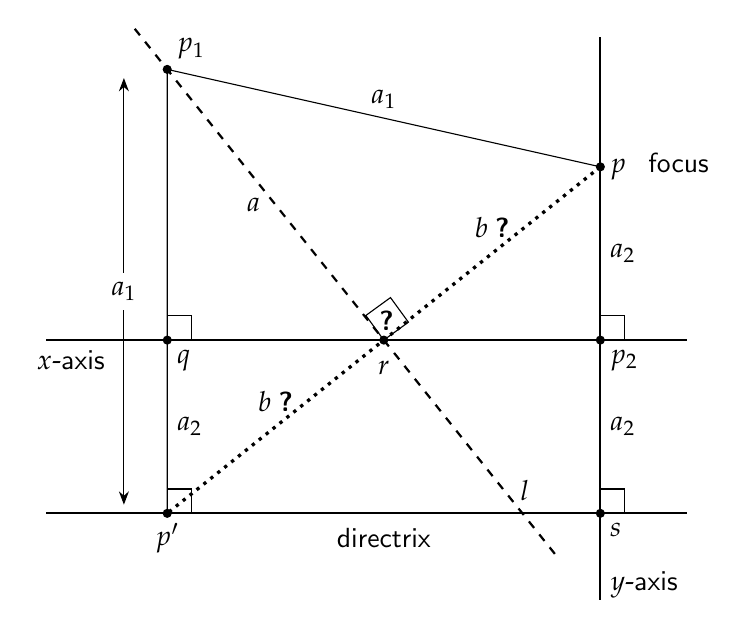
\begin{tikzpicture}[scale=1.1]
\draw[thick] (-6.4,0) -- node[very near start,below,xshift=-20pt] {$x$-\textsf{axis}} (1,0);
\draw[thick] (0,-3) -- node[very near start,right,yshift=-20pt] {$y$-\textsf{axis}} (0,3.5);
\draw[thick] (-6.4,-2) -- (1,-2);
\coordinate (F) at (0,2);
\fill (F) circle (1.5pt) node[right] {$p\;\;$ \textsf{focus}};
\fill (0,0) circle (1.5pt) node[below right] {$p_2$};
\coordinate (FP) at (-5,-2);
\fill (FP) circle (1.5pt) node[below] {$p'$};
\path (FP) -- node[below,yshift=-2pt] {\textsf{directrix}} (0,-2);
\fill (0,-2) circle (1.5pt) node[below right] {$s$};
\coordinate (F4) at (-5,3.125);
\fill (F4) circle (1.5pt) node[above right] {$p_1$};
\draw (F) -- node[right] {$a_2$} (0,0) -- node[right] {$a_2$} (0,-2);
\draw (F) -- node[above] {$a_1$} (F4) -- (FP);
\draw[<->] ($(F4)+(-.5,-.1)$) -- node[fill=white] {$a_1$}($(FP)+(-.5,.1)$);
\draw[thick,dashed] ($(F4)!-.15!(-2.5,0)$) -- node[very near end,right,xshift=2pt] {$l$} ($(F4)!1.8!(-2.5,0)$);
\draw[very thick,dotted] (F) -- (FP);
\coordinate (H) at (-2.5,0);
\node[above,xshift=1pt] at (H) {\textsf{\bfseries ?}};
\draw[rotate=36] (H) rectangle +(10pt,10pt);
\path (FP) -- node[above,yshift=2pt] {$b$ \textsf{\bfseries ?}} (H) -- node[above,yshift=2pt] {$b$ \textsf{\bfseries ?}} (F);
\draw (0,0) rectangle +(8pt,8pt);
\draw (0,-2) rectangle +(8pt,8pt);
\draw (-5,0) rectangle +(8pt,8pt);
\draw (-5,-2) rectangle +(8pt,8pt);
\fill (-5,0) circle (1.5pt) node[below right] {$q$};
\fill (-2.5,0) circle (1.5pt) node[below,yshift=-4pt] {$r$};
\path (-5,0) -- node[right] {$a_2$} (-5,-2);
\path (F4) -- node[left,xshift=-2pt] {$a$} (-2.5,0);
\end{tikzpicture}
\end{center}
\begin{itemize}
\item The directrix is parallel to the $x$-axis, the focus $p$ is on the $y$-axis and $\overline{p_1p'}$ is perpendicular to the directrix. Therefore, $\angle p'qr$ and $\angle pp_2r$ are right angles.
\item $\overline{qp'}$ and $\overline{p_2s}$ are opposite sides of a rectangle, so $\overline{qp'}=\overline{p_2s}$, which in turn is equal to $\overline{pp_2}$ since $p_2$ is on the parabola and thus equidistant from $p$ and $s$.
\item $\angle qrp'$ and $\angle p_2rp$ are equal vertical angles.
\item The right triangles $\triangle qrp'$ and $\triangle p_2rp$ have one acute angle equal and one side equal so they are congruent. Therefore, $\overline{p'r}=\overline{rp}$ and $\overline{p_1r}$ is the median of $\triangle pp_1p'$.
\item $p_1$ is on the parabola so $\overline{pp_1}=\overline{p_1p'}$. Therefore, $\triangle pp_1p'$ is an isoceles triangle.
\item In the isoceles triangle $\triangle pp_1p'$, the median $\overline{p_1r}$ is also the perpendicular bisector of $\overline{pp'}$.
\item Line $l$ contains the line segment $\overline{p_1r}$ and is the perpendicular bisector of $\overline{pp'}$.
\end{itemize}


\end{document}
